\documentclass{article}

%Headers
\usepackage[dvips]{graphicx}    %package that does pdfs
\usepackage{color}              %this needs to be here also
\usepackage{amssymb} %librerie simboli matematica
\usepackage{amsmath}

\usepackage{xcolor,listings} %per il codice
\usepackage{textcomp}
\lstset{upquote=true}

\usepackage{hyperref} %per gli hyperlink

\usepackage{imakeidx} %per l'indice
\makeindex



\title{Gran Compendio OLI}
\author{\href{https://github.com/meschio94/Gran-Compendio-OLI}{Meschio}}
\date{2021\\V1.0a}

\begin{document}
\maketitle

\begin{abstract}
Guida passo a passo per alcune tipologie di esercizi con immagini e ricche spiegazioni, frammenti di altri esercizi con casi particolari, il tutto organizzato per una facile consultazione in sede di esame o per apprendere i passaggi in fase di studio.\\
\\
Non è un sostituto all'esercizio e lo studio, l'esame richiede una buona dose di pratica e di comprensione teorica, l'uso esclusivo del compendio all'esame senza i punti precedenti vi porterà ad imparare una costosa ed evitabile lezione.
\end{abstract}

\tableofcontents

\section{Modelli}
Mi dispiace, qua non troverete guide per fare i modelli, sfortunatamente questi van fatti alla nausea cercando di capire di volta in volta e costruendosi il metodo, riporto solamente delle fattispecie di problemi con soluzioni di tipologie degne di nota.

\subsection{Cenni di Base}
\begin{itemize}
\item  Stiamo risolvendo problemi \textbf{lineari}, questo implica che non potete e non dovete moltiplicare due variabili che avete creato in nessun modo, è un errore molto grave, ad esempio:\\
$x_{ij} \{0,1\} $ e $y_i integer \geqq 0$, questa cosa è illegale: $\displaystyle \sum_{i \in J} x_{ij}y_i$\\
È comunque possibile moltiplicare tra loro parametri del problema e variabili create ad hoc da voi.
\item Il \textbf{Big M} è uno strumento che possiamo usare in certe circostanze, torna utile per impostare vincoli di verità, come ad esempio:\\
Supponiamo di dover produrre due prodotti A e B, il prodotto B ha una particolarità, nel caso ne facessimo anche solo 1, avremmo dei costi fissi $c_B$.\\
Ora noi impostiamo due variabili intere per rappresentare il numero di prodotti che stiamo producendo $x_A \geqq 0, integer$ e $x_B \geqq 0, integer$, ed una booleana per indicare se B è prodotto o no $y_B \in \{0,1\}$, come possiamo mettere un vincolo che nel caso in cui \textbf{NON} stiamo producendo B, allora per forza di cose $x_B$ dovrà essere $\leqq 0$ ?\\
$x_B \leqq My_B$\\
Perchè serve ? Perchè senza questo vincolo potrei avere $y_B=0$ e $x_B = 340 $, capite che qualcosa non funziona matematicamente.\\
Cosa stiamo facendo quindi? M rappresenta un numero molto grosso, nel momento in cui $y_B$ varrà 1, cioè stiamo producendo il prodotto B, avremo $x_B$ come intero positivo che sarà sempre minore di M, e il tutto rispetta il vincolo, nel caso in cui non produciamo B, $y_B$ varrà 0 che annullerà M, rendendo l'equazione $x_B \leqq 0$, quindi $x_B$ dovrà per forza essere 0 a sua volta ($x_B$ non può essere negativo dal vincolo messo sopra che la impone $\geqq 0$).
\item \textbf{L'opposto di una booleana} o \textbf{$(1-x_{ij})$}, questa è una chicca, serve per vedere la condizione opposta di uno stato di una booleana per un controllo inverso, vediamo un breve esempio:\\
Una azienda produce il prodotto X, la linea di produzione è formata da 3 differenti linee parallele identiche, 1,2,3, il prodotto X ha due lotti distinti, il lotto $\alpha$ e il lotto $\beta$, se produco il lotto $\alpha$ in una delle 3 linee, allora non posso produrre il lotto $\beta$ in quella linea.\\
Pongo $x_{ij} \in \{0,1\}, j \in \{1,2,3\}, i \in \{\alpha,\beta\} $ che rappresenta un booleano, che vale 1, nel caso in cui il lotto $i$ è prodotto nella linea $j$, 0 altrimenti.\\
Come posso fare il controllo di verità di questa condizione con un vincolo matematico ?\\
$\displaystyle \sum_{i \in \alpha} x_{ij} \leqq (1-x_{ki})M$ $i \in \{1,2,3\}, k \in \beta$\\
Sto ciclando a sinistra delal disuguaglianza tutti i prodotti X del lotto $\alpha$, la $j$ è vincolata fuori quindi guardiamo una linea alla volta, a destra della disuguaglianza sto dicendo che nel caso in cui $x_{kj}$ dove $k$ è l'insieme del lotto $\beta$ vale 1, quindi lo stiamo producendo nelal stessa linea produttiva $i$, allora avendolo posto negativo, si annulla con l'1 : $(1-x_{ki})$, valendo 0 e di conseguenza, rompendo il vincolo.\\
Il Big M a destra della parentesi, serve nel caso in cui non produciamo $\beta$ in quella specifica linea di produzione, e l'uno risultante dalla tonda che ne deriva, deve essere moltiplicato con qualcosa di grande per rendere vera l'equazione di sinistra.

\item \textbf{$\Delta$}, il delta viene usato per rappresentare la differenza di variabili, come può essere l'età media delle persone, se in un problema vedete un punto che risulta simile a:"minimizzare il valore assoluto della differenza massima tra l'etá media di un gruppo e un altro"

\item \textbf{Valore assoluto di un insieme $|A|$ }, è semplicemente un modo per esprimere il limite superiore di un insieme che non ha una definizione numerica, ad esempio se ho un insieme $A$ che rappresenta i nasi che ha un circo disponibile da allocare ai suoi clown, allora se pongo $x_i \geqq 0, integer$ come il numero totale di nasi che il gruppo di clown $i$ può prelevare, posso scrivere:\\
$x_i \leqq |A|$
\end{itemize}
\newpage
\subsection{Esercizi}
\subsubsection{Problema con Delta}
Esame 2020-07-16 Ex 1\\
\noindent\fbox{%
    \parbox{\textwidth}{%
In a summer camp there are 70 children to be allocated to 10 groups, each one
with an educator that must supervise exactly 7 children.\\
The age of each child is $e_i,i=1,\dots,70.$\\
We want to minimize the absolute value of the maximum difference between
the average age of a group and the age of each child allocated to that group (example: if the 7 children of a group have ages 8,9,10,11,11,12,12 the maximum
difference for this group is —73/7 - 8 = 2.43—).\\
Write an integer linear programming model in order to decide how to allocate
the children to the groups\\
Clearly define the used variables.
						}%
			}%
\\
Soluzione:\\
$x_{ig} = 1$ se il bimbo $i = 1,\dots,70$ è nel gruppo $g = 1 \in 10$, 0 altrimenti.\\
$\Delta$ massima differenza di età (valore assoluto).\\
\\
\begin{align*}
&min: \Delta\\
    	&\Delta \geqq \displaystyle \sum_{i = 1}^{70} \frac{e_i x_{jg}}{7} - e_j x_{jg} & &j=\{1,\dots,70\},g=\{1,\dots,10\}\\
    	&\Delta \geqq - \displaystyle \sum_{i = 1}^{70} \frac{e_i x_{jg}}{7} + e_j x_{jg} & &j=\{1,\dots,70\},g=\{1,\dots,10\}\\
    	&\displaystyle \sum_{g = 1}^{10} x_{ig} = 1 & &i=\{1,\dots,70\}\\
    	&\displaystyle \sum_{g = 1}^{70} x_{ig} = 7 & &g=\{1,\dots,10\}\\
    	&x_{ig} \in \{0,1\} & &i=\{1,\dots,70\},g=\{1,\dots,10\}\\
\end{align*}

\newpage
\subsubsection{Problema con massima distanza}
Esame 2020-06-25 Ex 1\\
\noindent\fbox{%
    \parbox{\textwidth}{%
A company that distributes medical products wants to open at least
1 out of 3 possible locations, to serve the set K of customers. $d_{ik}$ represents the distance from location $i$ to customer $k \in K$.
We want to decide which warehouse($s$) to open, and to assign each
customer to exactly one warehouse.
Write a MILP problem to minimize the maximum distance from a
customer to the assigned warehouse.
Clearly define the variables used.
						}%
			}%
\\
Soluzione:\\
$y_{ik} = 1$ se il cliente $k \in K$ è assegnato al magazzino $i$, 0 altrimenti.\\
$z_i=1$ se il magazzino nella località $i$ è aperto, 0 altrimenti.\\
$\alpha$ massima distanza.\\
\\
\begin{align*}
&min: \alpha\\
    	&\alpha \geqq d_{ik}y_{ik} & &i=1,2,3;k\in K\\
    	&\displaystyle \sum_{i = 1}^{3} z_i \geqq 1 \\
    	&\displaystyle \sum_{k \in K} y_{ik} \leqq |K|z_i & &i=1,2,3\\
    	&\displaystyle \sum_{i = 1}^{3} y_{ik} = 1 & &k \in K\\
    	&y_{ik} \in \{0,1\} & &i=1,2,3;k \in K\\
    	&z_{i} \in \{0,1\} & &i=1,2,3\\
    	&\alpha & &free
\end{align*}


\subsubsection{Problema Variabile Triplo indice}
Esame 2017-02-17 Ex 1\\
\noindent\fbox{%
    \parbox{\textwidth}{%
The national company for electric energy is going to plan the use of its
power generators for a time horizon $T$ of time periods. Let $N$ be the set of power generators
and let $M$ be the set of customers. For each customer $j \in M$ and each time period $t \in T$ it is known the forecasted demand $d_{jt}$. For each power generator $i \in N$ it is know the maximum power $P_i$ that can be produced in each time period, and the set $S(i) \subseteq M$ of the customers that may be served by generator $i$. A unit of energy produced by generator $i \in N$ in period $t \in T$ has a cost git. The energy produced by generator $i \in N$ can be transferred to customer $j \in M$ only if a $link$ has been established between $i$ and $j$. The installation of a link $(i, j)$ has cost $c_{ij}$ . To
have a robust service, in case of failure of a power generator, it is required that each customer is linked to at least 2 generators.\\
Write a linear program to help the company to define an optimal plan to install the links among generators and customers, and to provide the required energy to each customer, while minimizing the total cost.\\
Improve the above model by adding the following constraints: in each time period each customer can receive energy from no more than three generators;
						}%
			}%
\\
Soluzione:\\
$x_{ij} = 1$ se il generatore $i \in N$ è collegato al cliente $j \in S(i)$, 0 altrimenti.\\
$f_{ijt}=$ quantità di energia che il generatore $i$ da al cliente $j$, 0 altrimenti.\\
$\delta_{ijt}= 1$ se il generatore $i$ fornisce energia al cliente $j$ nel periodo $t$, 0 altrimenti.\\\\
\\
\begin{align*}
&min: z= \displaystyle \sum_{i \in N} \sum_{j \in S(i)} c_{ij}x_{ij} + \sum_{i \in N} \sum_{j \in S(i)}\sum_{t \in T}g_{it}f_{ijt}\\
    	&\sum_{i \in N:j \in S(i)}f_{ijt} \geqq d_{jt} & &\forall j \in M; \forall t \in T;\\
    	&\displaystyle \sum_{t \in T} f_{ijt} \leqq (|T|max_{t\in T} d_{jt})x_{ij} & &\forall i \in N,\forall j \in S(i) \\
    	&\displaystyle \sum_{j \in S(i)} f_{ijt} \leqq P_i & &\forall i \in N,\forall t \in T\\
    	&\displaystyle \sum_{i \in N: i \in S(i)} x_{ij} \geqq 2 & &\forall j \in M\\
		&f_{ijt} \leqq d_{jt}\delta_{ijt} & &\forall i \in N,\forall j \in S(i),\forall t \in T\\  
		&\displaystyle \sum_{i \in N} \delta_{ijt} \leqq 3 & &\forall j \in S(i),\forall t \in T\\
    	&x_{ij} \in \{0,1\} & &\forall i \in N,\forall j \in S(i)\\
    	&f_{ijt} \geqq 0 & &\forall i \in N,\forall j \in M,\forall t \in T\\
    	&\delta_{ijt} \in \{0,1\} & &\forall i \in N,\forall j \in S(i),\forall t \in T
\end{align*}

\subsubsection{Problema di Trasporto}
Esame 2018-01-11 Ex 1\\
\noindent\fbox{%
    \parbox{\textwidth}{%
The transport operator CITYFAST is specialized in good distribution in large metropolis. The distribution into the city requires two transports. A first transport from the suppliers (outside the city) to a city distribution center, and a second transport form the distribution center to the customers. Each supplier provides only one type of good. Let $I$ be the set of suppliers, $J$ the set of possible distribution centers and $K$ be the set of customers. The first transport is managed by an external company. CITYFAST pays $c'_{ij}$ euro for each kilogram transported from supplier $i \in I$ to distribution center $j \in J$. Instead, for the second transport, CITYFAST
uses its own fleet of identical ecological trucks, each with a given capacity $C$. The cost for a trip from the distribution center $j \in J$ to customer $k \in K$ (and return) is $c''_{ij}$. Each trip can deliver goods from several suppliers in order to use the truck capacity efficiently. Each trip serve a single customer. Each customer asks for $d_{ik}$ Kg of the good provided by supplier $i \in I$ (with $d_{ik}$ possibly zero if the good is not required). If a distribution center $j$ is used the company has to pay a fixed una-tantum amount of $s_j$ euro.\\
Help the company to find an optimal transport policy by writing a Linear Program aimed to satisfy all the demands, while minimizing the total cost. (Suggestion: use a three index variable
(supplier-distribution center-customer) to track the flows of goods.) Improve the previous model
by adding the following constraint: given a subset of customers: $A \subseteq K$, it is required that all the
customers of $A$ are served by a single distribution center which is the same for all these customers.
}%
			}%
\\
Soluzione:\\
$x_{ijk} =$ Kg del bene del fornitore $i$ trasportati da un centro di distribuzione $j$ al cliente $k$.\\
$y_{jk}=$ numero di viaggi dal centro di distribuzione $j$ al cliente $k$.\\
$\delta_j =$ 1 se il centro di distribuzione $j$ è usato, 0 altrimenti.\\
$M = $ un numero molto grande (costante).\\
$z_{jk}$ 1 se il centro di distribuzione $j$ serve il cliente $k \in A$, 0 altrimenti.\\
\\
\begin{align*}
&min: z= \displaystyle \sum_{j \in J}s_j\delta_j + \sum_{i \in I} \sum_{j \in J} \sum_{k \in K} c'_{ij}x_{ijk} + \displaystyle \sum_{j \in J} \sum_{k \in K}c''_{jk}y_{jk} & &k \in K, i \in I\\
		&\displaystyle \sum_{j \in J}x_{ijk} = d_{ik} & &k \in K, i \in I\\
    	&\displaystyle \sum_{i \in I}x_{ijk} \leqq Cy_{jk} & &k \in K, j \in J\\
    	&\displaystyle \sum_{i \in I} \sum_{k \in K} x_{ijk} \leqq M \delta_j & &j \in J \\
    	&x_{ijk} \geqq 0 & &i \in I, j \in J, k \in K\\
    	&y_{jk} \geqq 0, integer & &j \in J, k \in K\\
    	&\delta_{j} \in \{0,1\} & &j \in J\\
    	&y_{jk} \leqq Mz_{jk} & &k \in A, j \in J\\
    	&\displaystyle \sum_{j \in J} z_{jk} = 1 & &k \in A\\
    	&z_{jk} = z_{jh} & &k,h\in A, j \in J\\
\end{align*}

\newpage
\subsubsection{Problema di Stoccaggio}
Esame 2017-07-17 Ex 3\\
\noindent\fbox{%
    \parbox{\textwidth}{%
A tile factory wants to organize the storage area of the pallets containing final products. There
is a set $I$ of pallets that have to be stored in a set $L$ of possible locations. In each location one
can store up to $m$ pallets one over the other. Over each pallet of a special ”fragile” set $F$ one
can store at most two pallets.\\
Write a linear programming model to help the factory to find a feasible storage for all pallets
(without objective function).\\
Let $\sigma$ denote a sorting of the the pallets, i.e., $\sigma(i) < \sigma(j)$ indicates that pallet $i$ precedes
pallet $j$. In a second time the pallets will be picked from the storage area one after the other
accordingly to the above ordering. If pallet i with $\sigma(i) < \sigma(j)$ is stored under pallet $j$ (in the
same location) before picking i one must move pallet $j$. Improve the linear programming model
by adding an objective function which minimizes the movement of pallets.

}%
			}%
\\
Soluzione:\\
$x_{ilk} = 1$ se il pallet $i$ è stoccato nella locazione $l$ al livello $k$, 0 altrimenti.\\
$y_{ij}=1 $ se il pallet è sotto al pallet $j$ (stessa location), 0 altrimenti.\\
\begin{align*}
&min: z= \displaystyle \sum_{i \in I} \sum_{j \in I: \sigma(i)<\sigma(j)} y_{ij}\\
		&\displaystyle \sum_{l \in L}\sum_{k=1}^{m}x_{ilk} = 1 & &i \in I\\
    	&\displaystyle \sum_{i \in I} x_{ilk} \leqq 1 & &l \in L,k=1,\dots,m \\
    	&\displaystyle \sum_{i \in I} x_{ilk} \geqq \sum_{i \in I} x_{il(k+1)} & &l \in L,k=1,\dots,m-1 \\
    	&\displaystyle m(1-x_{ilk}) \geqq \sum_{h=k+1}^{m} \sum_{j \in I:j \neq i} x_{ilh}-2 & &i \in F,l \in L,k=1,\dots,m-3 \\
    	&\displaystyle x_{ilk}  \sum_{h=k+1}^{m} x_{jlk} - 1  \leqq y_{ij} & &i,j \in I,i \neq j,l \in L,k=1,\dots,m-1 \\
    	&x_{ilk} \in \{0,1\} & &i \in I, l \in L,k=1,\dots,m\\
    	&y_{ij} \in \{0,1\} & &i,j \in I, i \neq j\\
\end{align*}

\subsubsection{Problema di Stoccaggio 2}
Esame 2020-06-08 Ex 2\\
\noindent\fbox{%
    \parbox{\textwidth}{%
A warehouse has to store n boxes in a rack with $m$ shelves. The first
$m1$ shelves have length $L1$, while the remaining have length $L2$. Each
box $j-1,\dots,n$ has length $l_j$ and a frequency of usage $f_j$.\\ 
Write a linear programming model that helps the warehouse to decide how to
store the boxes, so that the sum of the frequencies of the boxes stored
in the first $m1$ shelves is maximized. (N.B. It is not known if all the
boxes can be stored.)

}%
			}%
\\
Soluzione:\\
$x_{ij} = 1$ se la scatola $j$ è stoccata nello scaffale $i$, 0 altrimenti.\\
\begin{align*}
&max: z= \displaystyle \sum_{i = 1}^{m1} \sum_{j = 1}^{n} x_{ij}f_j\\
		&\displaystyle \sum_{i=1}^{m}x_{ij} \leqq 1 & &j = 1,\dots,n\\
    	&\displaystyle \sum_{j = 1} l_{j}x_{ij} \leqq L1 & &i=1,\dots,m1 \\
    	&\displaystyle \sum_{j = 1} l_{j}x_{ij} \leqq L2 & &i=m1+1,\dots,m \\
    	&x_{ij} \in \{0,1\} & &i=1,\dots,m,j=1,\dots,n\\
\end{align*}

\newpage
\section{Forme: Standard, Canonica, Generale}
I problemi di LP possono essere rappresentati a sistema con 3 differenti forme, tutte equivalenti.\\
\begin{itemize}
\item \textbf{Standard}
\begin{itemize}
\item $min\{c^Tx:Ax=b,x_j \geqq 0, j=1,\dots,n \}$
\item I vincoli sono uguaglianze "$=$", tutte le variabili hanno vincoli di non negatività.
\end{itemize}

\item \textbf{Canonica}
\begin{itemize}
\item $min\{c^Tx:Ax \geqq b,x_j \geqq 0, j=1,\dots,n \}$
\item I vincoli sono disuguaglianze "$\geqq$,$\leqq$", tutte le variabili hanno vincoli di non negatività.
\end{itemize}

\item \textbf{Generale}
\begin{itemize}
\item $min\{c^Tx:Ax = b, A'x \geqq b, x_j \geqq 0, j \in J \subset \{1,\dots,n\} \}$
\item I vincoli sono disuguaglianze "$\geqq$,$\leqq$" e uguaglianze "$=$", solo le variabili del sotto insieme $J$ devono essere non-negative.
\end{itemize}
\end{itemize}

\subsection{Standard $\Rightarrow$ Canonica}
Le uguaglianze, diventano disequazioni:

\begin{align*}
2x_1 + 5x_2 = 4 & \Rightarrow  \left\{ \begin{array}{rcl} 2x_1 + 5x_2 \geqq 4 \\ 2x_1 + 5x_2 \leqq 4 \end{array}\right.
\end{align*}
\subsection{Generale $\Rightarrow$ Standard}
Le disuguaglianze diventano uguaglianze:
\begin{align*}
5x_1 + 3x_2 \leqq 4 & &\Rightarrow & &2x_1 + 5x_2 + S_1 = 8, S_1 \geqq 0
\end{align*}
$S_1$ è variabile di slack, che serve per bilanciare la disequazione, in questo altro esempio non sarebbe servita:
\begin{align*}
5x_1 + 3x_2 \geqq 4 & &\Rightarrow & &2x_1 + 5x_2 = 8
\end{align*}

\subsection{Esercizio Trasformazione Gran Fritto Misto}
Esame 2020-06-25 Ex 3\\
\noindent\fbox{%
    \parbox{\textwidth}{%
Consider this minimization problem:\\
\begin{align*}
mix:  &8x_1 + 3x_2 + x_3 \\
    	&2x_1 + 7x_2 - 5x_3 = 4\\
    	&4x_1 - 3x_2 + x_3 \geqq 8\\
    	&x_1 \geqq 0\\
    	&x_2 \leqq 0\\
    	&x_3  free
\end{align*}
Write the corresponding canonical form.
	}%
}%
\\
Soluzione:\\
\begin{align*}
mix:  &8x_1 + 3x_2 + x_3^+ - x_3^- \\
    	&2x_1 - 7x_2 - 5x_3^+ + 5x_3^- \geqq 4\\
    	&-2x_1 + 7x_2 + 5x_3^+ - 5x_3^- \geqq -4\\
    	&4x_1 + 3x_2 + x_3^+ -x_3^- \geqq 8\\
    	&x_1,x_2,x_3^+,x_3^- \geqq 0
\end{align*}
Le variabili free son state sdoppiate, $x_3 \Rightarrow x_3^+,x_3^-$ e sostituite nel sistema, la $x_3^+$ ha mantenuto sempre il suo segno, mentre la $x_3^-$ aveva l'opposto della sua controparte positiva.\\
Nel secondo vincolo avevamo un uguaglianza, abbiamo quindi dovuto porre il segno a $\geqq$ e aggiungere una nuova riga, con gli stessi termini moltiplicati per $-1$ e segno $\leqq$.

\newpage
\section{Matrici : LP, ILP}

\subsection{Fondamenti Concettuali}
\subsubsection{Quale Simplesso?}
Quale simplesso dovrei usare se il professore non lo specifica ?\\
Abbiamo 3 strumenti, che non sono equivalenti (quasi), vediamo la mappa concettuale:\\

\begin{center}
\raisebox{-.5\height}{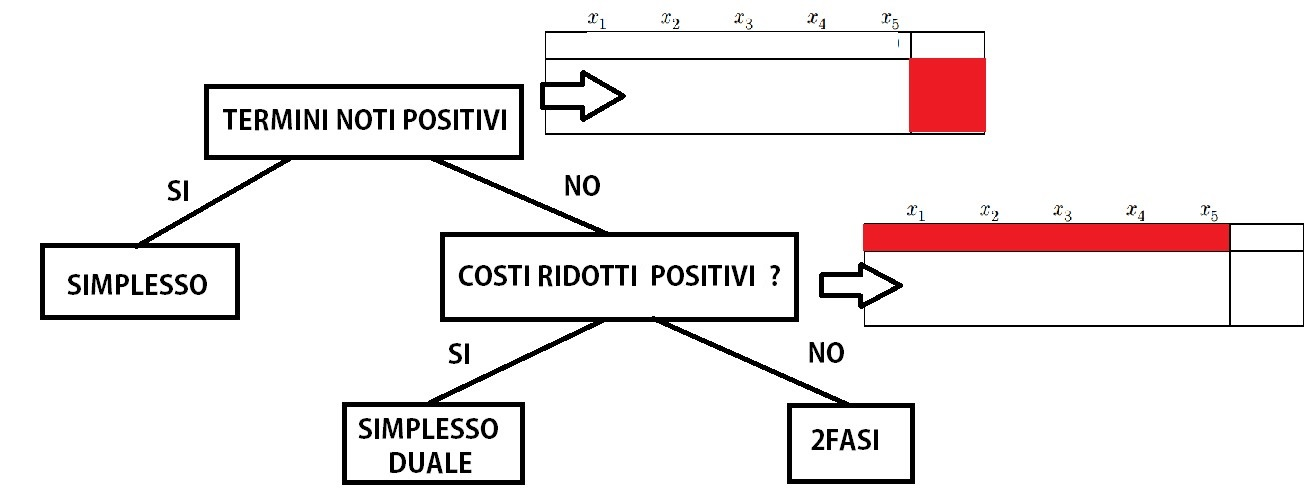
\includegraphics[width=12cm]{immagini/mappa.jpg}}
\end{center}

Questo sarebbe il flusso logico per approcciare il problema, in realtà il 2fasi può sempre sostituire il simplesso duale, non è vero il contrario, in ogni caso il 2 fasi essendo più lungo è sconveniente usarlo sempre.
NB. La condizione di scelta del primo ramo no (costi ridotti negativi), non è discriminante della radice (termini noti positivi), ovvero, il simplesso standard, \underline{può} essere usato se i suoi costi ridotti sono negativi, è condizione necessaria che abbia i termini noti positivi.
\subsection{LP}
Linear Programming, in italiano Programmazione Lineare PL
\subsubsection{Simplesso}
una volta che abbiamo sviluppato il nostro problema e sistemato i vincoli, trovandoci nella condizione di poterlo sfruttare avendo i termini noti positivi una volta costruito il tableu, le iterazioni per selezionare il pivot saranno le seguenti:\\
\begin{itemize}
\item Siamo in un problema di $Massimo$: Scelgo le colonne che hanno valori $positivi$,non do precedenza a nessuna colonna specifica se ne incontro più di una $positiva$, prendo sempre quella più a sinistra, con indice minore (legge di Bland).


\item Siamo in un problema di $Minimo$: Scelgo le colonne che hanno valori $negativi$,non do precedenza a nessuna colonna specifica se ne incontro più di una $negativa$, prendo sempre quella più a sinistra, con indice minore (legge di Bland).

\end{itemize}

Una volta designata la colonna, la riga viene scelta prendendo il valore $minore$ dal rapporto dato da $\frac{b_i}{a_{ic}}$, dove $i$ è l'indice di riga, $c$ è l'indice di colonna e $b$ è il termine noto della riga $i$ che stiamo analizzando, come da esempio nell'immagine:\\

\begin{center}
\raisebox{-.5\height}{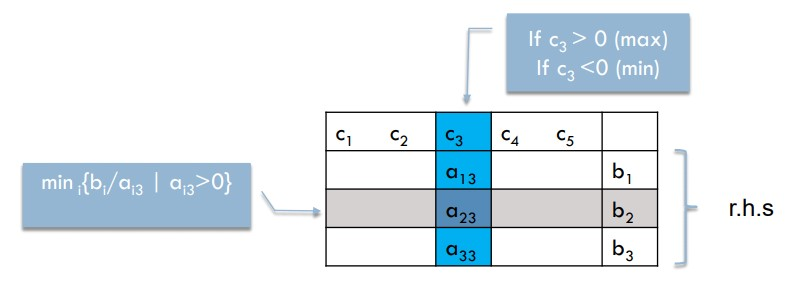
\includegraphics[width=12cm]{immagini/PivotSimplex.jpg}}
\end{center}

È importante notare che $a_{ic} > 0$, affinchè il tutto funzioni.\\
Iteriamo finchè la riga della funzione obbiettivo, ovvero la $R0$ (o anche riga dei costi), non diventa tutta $positiva$ se siamo in problema di $minimo$, o $negativa$ se siamo in un problema di $massimo$.

\subsubsection{Simplesso Duale}
Il processo è molto simile al Simplesso standard, con una sostanziale differenza, ora non partiamo più a selezionare la colonna in base a che tipo di problema di ottimizzazione ci troviamo ($max$ o $min$), ma prima partiamo a scegliere la riga, in base al fatt oche il termine noto sia negativo (vale per entrambi i problemi):\\
\begin{center}
\raisebox{-.5\height}{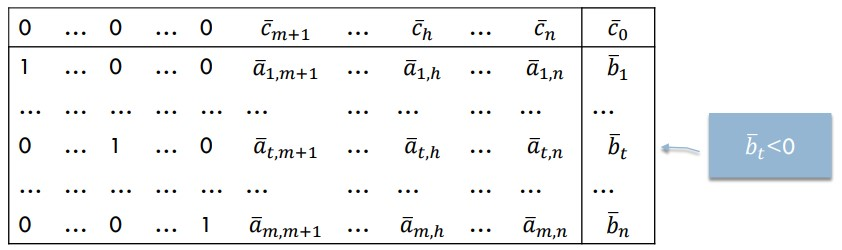
\includegraphics[width=10cm]{immagini/DualSimplex0.jpg}}
\end{center}

Una volta scelta la riga, devo scegliere solo i valori di quella riga che sono $negativi$, affinchè nel momento in cui farò diventare 1 quel pivot, il termine noto rispettivo $\overline{b}_t$ diventi anch'esso positivo, nel caso in cui non ci siano valori negativi nella riga, allora il duale è illimitato e ci fermiamo.\\

\begin{center}
\raisebox{-.5\height}{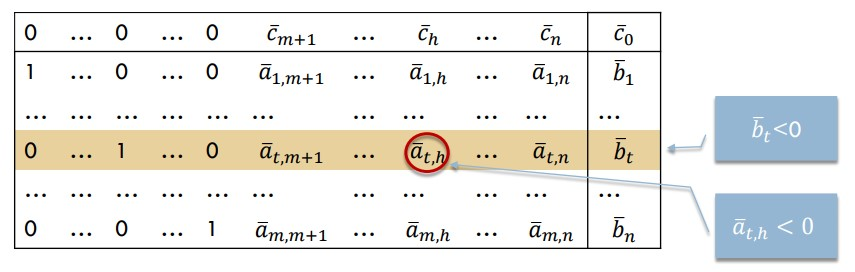
\includegraphics[width=10cm]{immagini/DualSimplex1.jpg}}
\end{center}

Nel caso avessi più di un valore negativo da cui scegliere, scelgo il pivot che ha un rapporto minore tra il valore della colonna, fratto il relativo pivot: $\frac{\overline{c}_j}{|\overline{a}_{t,j}|}$\\

\begin{center}
\raisebox{-.5\height}{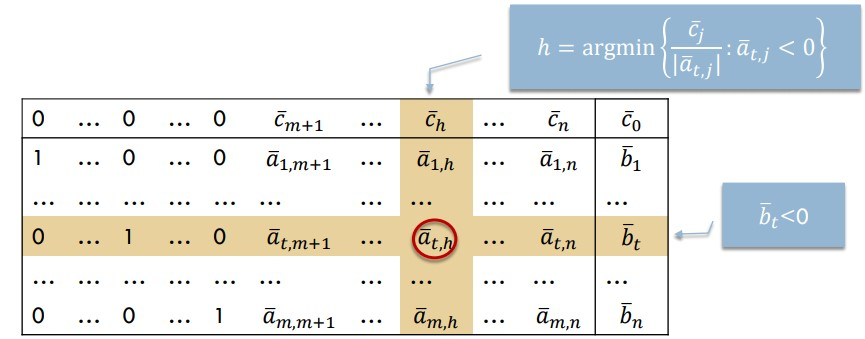
\includegraphics[width=10cm]{immagini/DualSimplex2.jpg}}
\end{center}
Continuo ad iterare fintanto che i termini noti non sono tutti positivi.\\
NB. È importante che la $R_0$ rimanga sempre positiva, perchè è condizione necessaria del simplesso duale.

\subsubsection{2Fasi}
Il metodo delle due fasi può sostituire il simplesso duale, nel caso in cui noi avessimo dei termini noti negativi, sarebbe sufficiente cambiare i segni dei vincoli, in modo da forzarli positivi, e bilanciare le slack negative con le variabili di surplus, il 2 fasi \underline{richiede} in input un problema di $minimizzazione$, quindi nel caso in cui avessimo un problema di massimo, cambiamo i segni di quella riga per ricondurci all'input adeguato.\\

\begin{center}
\raisebox{-.5\height}{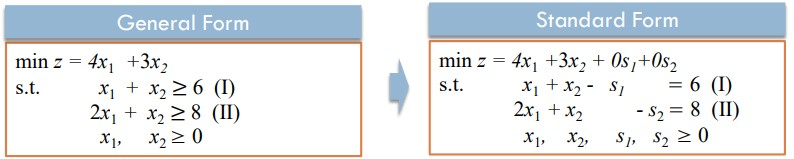
\includegraphics[width=12cm]{immagini/2fasi0.jpg}}
\end{center}

Dal nome, ci sono due fasi principali su cui lavorare, partiamo dalla prima fase, dobbiamo costruire un tableu una volta ricavata la forma standard, poniamo a 0 tutti gli elementi della $R_0$, lasciando un 1 esclusivamente dove è presente una variabile di surplus.
Le variabili di surplus vengono aggiunte solo se la slack di quel vincolo è negativa.

\begin{center}
\raisebox{-.5\height}{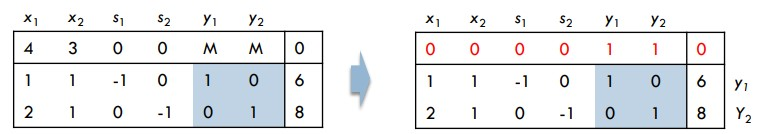
\includegraphics[width=12cm]{immagini/2fasi1.jpg}}
\end{center}

Procediamo facendo sparire gli $1$ delle rispettive variabili di surplus dalla $R_0$:\\

\begin{center}
\raisebox{-.5\height}{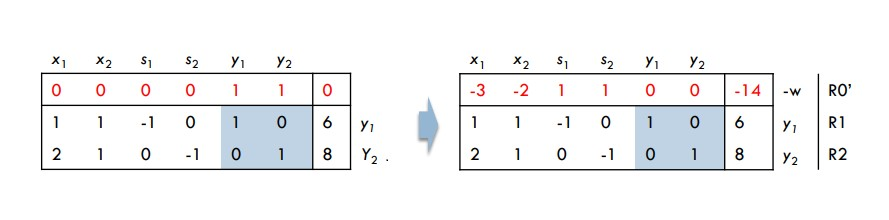
\includegraphics[width=12cm]{immagini/2fasi2.jpg}}
\end{center}


Adesso procediamo iterando con il simplesso standard, quindi, trovandoci in un problema di minimizzazione, dobbiamo far sparire le colonne che nella $R_0$ hanno valori $negativi$.\\

\begin{center}
\raisebox{-.5\height}{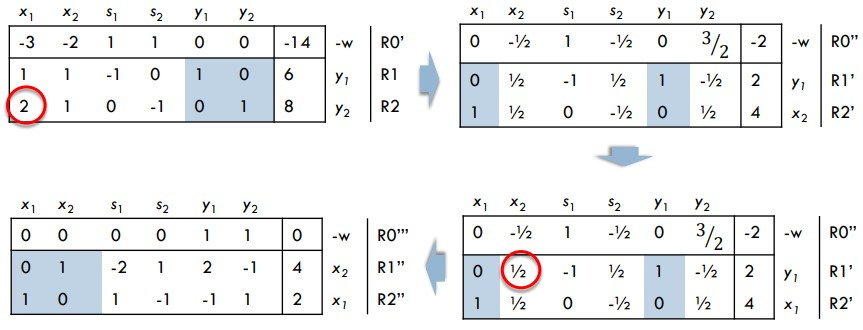
\includegraphics[width=12cm]{immagini/2fasi3.jpg}}
\end{center}

Iniziamo ora la \underline{Seconda Fase}, prendiamo la matrice precedente che ora si trova la $R_0$ piena di 0 ad esclusione delle colonne delle variabili di surplus, rimuoviamo quindi queste colonne e sostituiamo la $R_0$ con le variabili della funzione obbiettivo del problema originale.
NB.Se il problema era di massimizzazione originariamente, dobbiamo riportarcelo, nel caso fosse di minimizzazione possiamo lasciarlo così com'è.\\
\begin{center}
\raisebox{-.5\height}{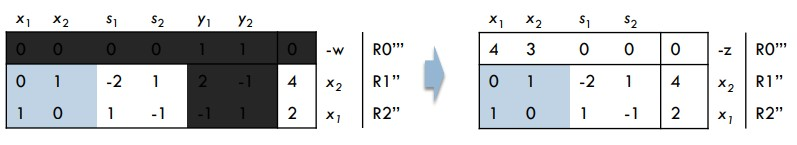
\includegraphics[width=12cm]{immagini/2fasi4.jpg}}
\end{center}

Procediamo infine ad avere gli 0 nelle rispettive colonne della nostra base, in modo da sviluppare la soluzione, quindi tramite operazioni matriciali sistemiamo la $R_0$.\\

\begin{center}
\raisebox{-.5\height}{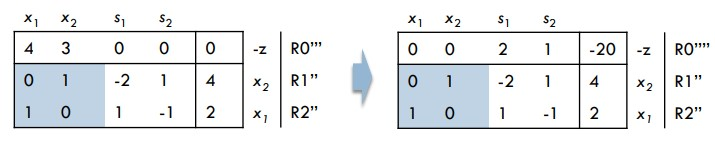
\includegraphics[width=12cm]{immagini/2fasi5.jpg}}
\end{center}

\subsubsection{Duale del problema}
Come trasformiamo il nostro sistema in un problema duale ?\\
Per prima cosa dobbiamo scegliere una direzione per i segni, tutti devono andare nella stessa direzione (non va considerata la riga finale delle $x_i \geqq 0$ ), Esempio:\\


\begin{align*}
min: &2x_1 + 3x_2 + x_3      &              &          min:& &2x_1 + 3x_2 + x_3\\
&-x_1 + 3x_2 - 2x_3 \geqq 8  & \Rightarrow  &                & &-x_1 + 3x_2 - 2x_3 \geqq 8\\
&x_2 - x_3 \leqq 2           &              & 			     & &-x_2 + x_3 \geqq -2\\
&x_1, x_2,x_3 \geqq 0        &              & 				 & &x_1, x_2,x_3 \geqq 0\\
\end{align*}

Ordiniamo il sistema per una maggiore chiarezza:\\

\begin{center}
\raisebox{-.5\height}{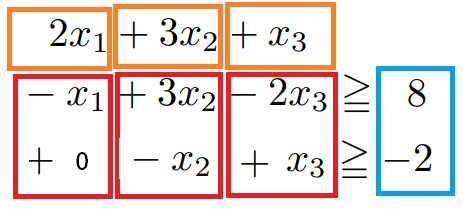
\includegraphics[width=8cm]{immagini/DualeProblema.jpg}}
\end{center}

Possiamo dividerlo in sotto vettori colonna, prendendo il vettore colonna delle $x_1$, partiamo dal vettore colonna dei vincoli, evidenziata di rosso, ribaltiamo di 90 gradi a sinistra e sostituiamo ogni $x$ con $u_i$ dove $i$ rappresenta la riga del vettore colonna, quindi avremo:\\
$-u_1 + 0u_2$ $\Rightarrow$ $-u_1$\\
mettiamo ora la disequazione, che rappresenta il verso opposto a quello scelto precedentemente, quindi avevamo impostato il sistema tutto a: $\geqq$, avremo:\\
$-u_1 \leqq$\\
A destra della disequazione inseriamo il vettore colonna arancione, ovvero il valore della rispettiva $x_1$ della funzione obbiettivo:\\
$-u_1 \leqq 2$\\
Reiteriamo per ogni colonna, il vettore colonna azzurro, ovvero il vettore dei termini noti, sarà la nostra nuova funzione obbiettivo, usiamo lo stesso procedimento di prima, quindi avremo $8u_1 - 2u_2$, il problema verrà anche invertito quindi dal $minimo$ di partenza, ora averemo un $massimo$:\\

\begin{center}
\begin{align*}
max: &8u_1 - 2u_2 \\
&-u_1 \leqq 2  \\
&3u_1 - u_2 \leqq 3   \\
&-2u_1 + u_2 \leqq 1   \\
&u_1, u_2 \geqq 0 \\
\end{align*}

\raisebox{-.5\height}{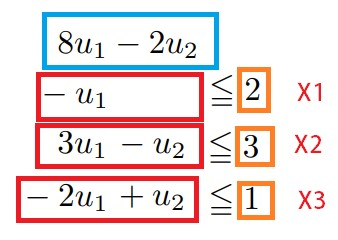
\includegraphics[width=5cm]{immagini/ProblemaDuale1.jpg}}
\end{center}

Osservando l'ultima immagine per chiarezza col risultato finale che si riconduce al sistema iniziale.

\subsection{Rappresentazione Grafica}
Anche tu sei a digiuno di grafici ed hai un incontrollato appetito di disegnarne altri ?\\
Molto semplicemente partendo da un sistema, si calcola la derivata prima della funzione obbiettivo per avere il nostro bel gradiente.
Ogni vincolo è una retta nel grafico e il segno è l'area accettabile dove guardare, un esempio semplice di un problema duale:\\
\begin{align*}
max: &8u_1 - 2u_2 \\
&-u_1 \leqq 2  \\
&3u_1 - u_2 \leqq 3   \\
&-2u_1 + u_2 \leqq 1   \\
&u_1, u_2 \geqq 0 \\
\end{align*}
Possiamo interpretare per facilità gli $u_1$ come $x$ e gli $u_2$ come $y$, avremo un gradiente : $\nabla = (8,-2)$.\\
prendiamo il primo vincolo: $-u_1 \leqq 2$ $\Rightarrow$ $-x \leqq 2$\\
Quindi ponendo $x=0$ non salta fuori nulla.\\
Il secondo vincolo $3x -y \leqq 3$, ponendo $x=0$ ricavo il primo punto $y= -3$
con $\geqq $ avendo cambiato il segno,coem secondo punto per tracciare la retto scelgo $x=1$, avrò $y=0$ sempre con $\geqq $, traccio al retta nel grafico.\\
Ultimo vincolo $-2x +y \leqq 1$, pongo $x=0$ avrò $y = 1$ con l'area acettabile sotto di essa $\leqq 1$, secondo punto pongo $x=-\frac{1}{2}$ avrò $y=0$, il grafico risultante qua sotto, ha l'area interna ammissibile, che si trova nel primo quadrante del grafico, avendo come vincolo ulteriore $u_1,u_2 \geqq 0$, dal gradiente che cade sul punto 8 in questo caso, la soluzione ottimale è lo spigolo in alto a destra con coordinate $(4,9)$ che corrisponde alla soluzione $z = 30$ andando a sostituire le coordinate nella funzione obbiettivo di max del problema.
\begin{center}
\raisebox{-.5\height}{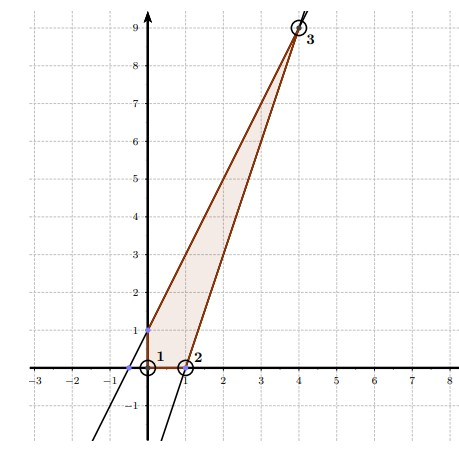
\includegraphics[width=9cm]{immagini/Grafico1.jpg}}
\end{center}
\subsection{ILP}
Integer Linear Programming, in italiano Programmazione Lineare Intera PLI
\subsubsection{Tagli di Gomory}
I tagli di gomory si usano quando il nostro problema da PL Lineare è PLI, ovvero Lineare Intero, il principio è che, non avendo numeri con virgole, posso approssimare il risultato all'intero più vicino.\\

Partendo dal tableu già risolto e con risultato ottimale e avendo termini fratti nella $R_0$, posso sfruttare Gomory per trovare una soluzione PLI, la formula da usare è:\\
$\displaystyle \sum_{j \in F} ( \underline{a}_{tj} - \lfloor \underline{a}_{tj} \rfloor )x_j \geqq \underline{b}_t -  \lfloor \underline{b}_t \rfloor$

NB. Le sbarre non sono valore assoluto, ma significano che approssimo difetto.\\
Dovrò aggiungere una riga e una colonna alla fine del mio tableu, sfruttando la relativa formula, vediamo un esempio:\\

\begin{center}
\raisebox{-.5\height}{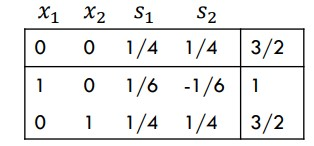
\includegraphics[width=6cm]{immagini/Gomory0.jpg}}
\end{center}

\begin{itemize}
\item Prendiamo una riga che abbia un termine noto frazionario, in questo caso $R_2$
\item Scriviamo : $x_2 + \frac{1}{4} S_1 + \frac{1}{4} S_2 = \frac{3}{2}$
\item usiamo al formula di Gomory: $  ( \frac{1}{4} - \lfloor \frac{1}{4} \rfloor )S_1 +  ( \frac{1}{4} - \lfloor \frac{1}{4} \rfloor )S_2 \geqq ( \frac{3}{2} - \lfloor \frac{3}{2} \rfloor )$
\item effettuiamo gli arrotondamenti: $  ( \frac{1}{4} - 0 )S_1 +  ( \frac{1}{4} - 0 )S_2 \geqq ( \frac{3}{2} - 1 )$
\item arriviamo a: $\frac{1}{4}S_1 + \frac{1}{4}S_2 \geqq \frac{1}{2}$
\end{itemize}

Possiamo ora inserire la riga nel tableu, aggiungendo anche una colonna di surplus per bilanciare:\\

$\frac{1}{4}S_1 + \frac{1}{4}S_2 -S_3 = \frac{1}{2}$

NB. la Slack $S_3$ è negativa perchè il segno era $\geqq$, fosse stato $\leqq$ sarebbe stata positiva.\\
Moltiplichiamo per $-1$ la riga per avere una base accettabile:\\
\begin{center}
\raisebox{-.5\height}{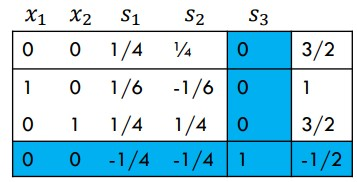
\includegraphics[width=6cm]{immagini/Gomory1.jpg}}
\end{center}

La seguente soluzione non è accettabile per il costo negativo dei termini noti ($-\frac{1}{2}$), dalla sezione del Compendio 2.1.1 sappiamo che dobbiamo usare il simplesso Duale, iteriamo di conseguenza:\\

\begin{center}
\raisebox{-.5\height}{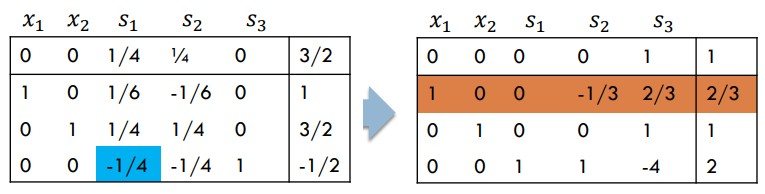
\includegraphics[width=9cm]{immagini/Gomory2.jpg}}
\end{center}

Ora la base è accettabile, abbiamo però un nuovo valore frazionario nei termini noti , $R_1$, possiamo iterare di nuovo con gomory seguendo il procedimento precedente:\\

$  ( -\frac{1}{3} - \lfloor - \frac{1}{3} \rfloor )S_2 +  ( \frac{2}{3} - \lfloor \frac{2}{3} \rfloor )S_3 \geqq ( \frac{2}{3} - \lfloor \frac{2}{3} \rfloor )$  $\Rightarrow$  $( \frac{1}{3} + 1 )S_2 +  ( \frac{2}{3} - 0 )S_3 \geqq ( \frac{2}{3} - 0 )$\\
NB. L'arrotondamento di $S_2$ è stato di $+1$, i termini negativi, per difetto, si avvicinano a $- \infty$, di conseguenza $- \frac{1}{3} \Rightarrow -0,33 \Rightarrow -1 $ !\\
Avremo: $\frac{2}{3}S_2 + \frac{2}{3}S_3 -S_4 = \frac{2}{3}$

Aggiungiamo la riga nel tableu moltiplicandola prima per $-1$ come prima:\\

\begin{center}
\raisebox{-.5\height}{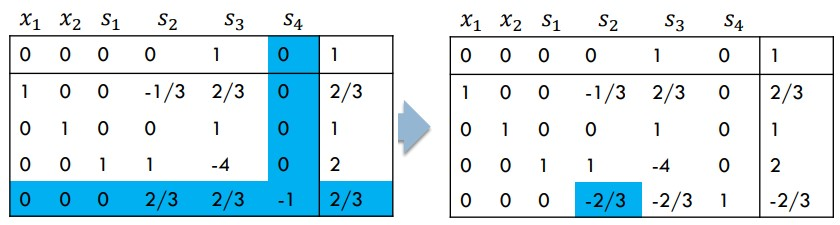
\includegraphics[width=9cm]{immagini/Gomory3.jpg}}
\end{center}

E risolviamo con il simplesso duale vista la situazione, qua il risultato finale:\\

\begin{center}
\raisebox{-.5\height}{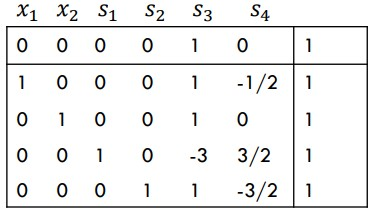
\includegraphics[width=6cm]{immagini/Gomory4.jpg}}
\end{center}

La soluzione infine è: $(x|s)*=(1,1,1,1,0,0), z^* = -1$






\subsection{Esercizi Particolari}
\subsubsection{Simplesso con variabili free}
Esame 2018-07-19 Ex 2\\
\noindent\fbox{%
    \parbox{\textwidth}{%
Consider the following PLC problem. Solve it with the simplex method, using the Bland’s rule.
Verify the solution by solving the problem with the graphic method.

\begin{center}
\begin{align*}
max: 	&x_1 - 2x_2\\
	 	&x_1 - x_2 \leqq 1\\
		&-2x_1 + x_2 \leqq 1\\
		&x_1,x_2 free\\
\end{align*}
\end{center}
						}%
			}%
\\
Soluzione: \\
Prima di partire notiamo che le x sono free, questo comporta una particolarità, dobbiamo vincolarle $\geqq 0$, scriveremo :\\
\begin{center}
\begin{align*}
max: &x_1^+ - x_1^- -2x_2^+ + 2x_2^-\\
&x_1^+ -x_1^- - x_2^+ + x_2^- \leqq 1\\
&-2x_1^+ + 2x_1^- + x_2^+ -x_2^- \leqq 1\\
&x_1^+ ,x_1^-,x_2^+,x_2^- \geqq 0\\
\end{align*}
\end{center}

costruiamo il relativo tableu e risolviamolo con il simplesso standard:\\

\begin{center}
\raisebox{-.5\height}{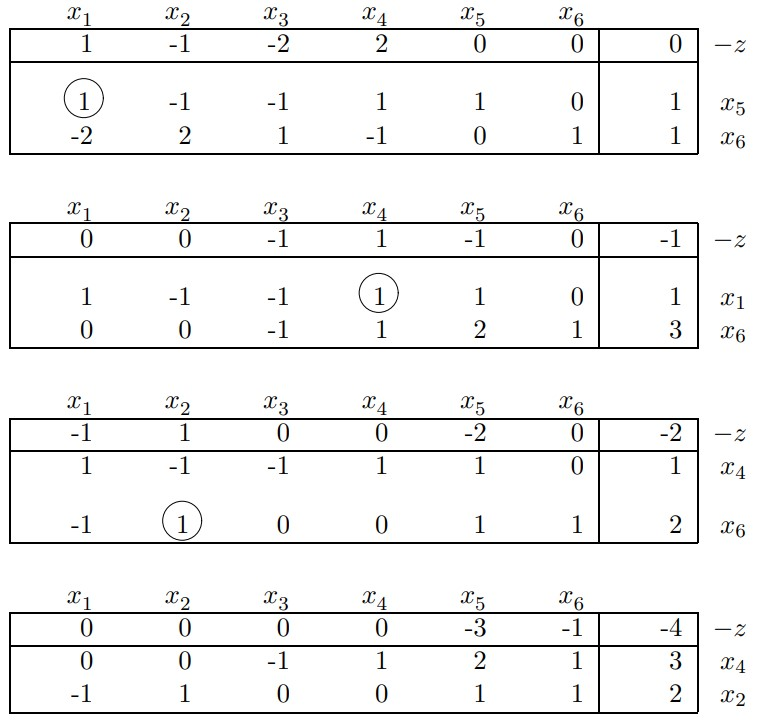
\includegraphics[width=10cm]{immagini/matrici/2_0_1_0.jpg}}
\end{center}

NB. Perchè nella prima matrice prendo come pivot $1$ invece di $-2$ ?\\
Ricordando dalla sezione del Compendio $2.1.2$, il valore del pivot deve essere $>0$, $-2$ non soddisfa questo requisito.\\
Arrivati alla fine, come soluzione avremo le colonne $x_4$ che rappresenta $x_2^-$ e la colonna $x_2$ che rappresenta $x_1^-$, avremo perciò:\\
$x_1^-=2 \Rightarrow x_1 = -2$ \\
$x_2^-=3 \Rightarrow x_2 = -3$\\
$z = 4$\\
cambiamo semplicemente i segni essendo che sono le $x^-$\\

\newpage
\subsubsection{Problema PLC con simplesso e gomory in salsa teriyaki}
In questo esercizio ci sta la particolarità che il sistema viene già impostato a $ = $ senza disequazioni, non si sa perchè, ma sembra funzionare, si usa il due fasi e si aggiungono alla cazzo di cane le colonne di surplus perchè sì, come punto aggiuntivo ci sta anche da usare i tagli di Gomory:\\
Esame 2017-02-17 Ex 2\\
\noindent\fbox{%
    \parbox{\textwidth}{%
 Consider the following PLC problem. Solve it with the simplex method.\\
\begin{center}
 
\begin{align*}
min:  &x_1 + 2x_2 + 1x_3 \\
    	&2x_1 + 3x_2 - 2x_3 = 20\\
    	&x_1 - 2x_2 + 3x_3 = 12\\
    	&x_1,x_2,x_3 \geqq 0\\
\end{align*}

\end{center}

Add the integrality constraints for the variables x and apply the cutting plane method with
Gomory’s cuts to look for an integer solution. Always choose the first row available to generate
a cut. Stop the algorithm after adding at most two cuts
	}%
}%

\begin{center}
\raisebox{-.5\height}{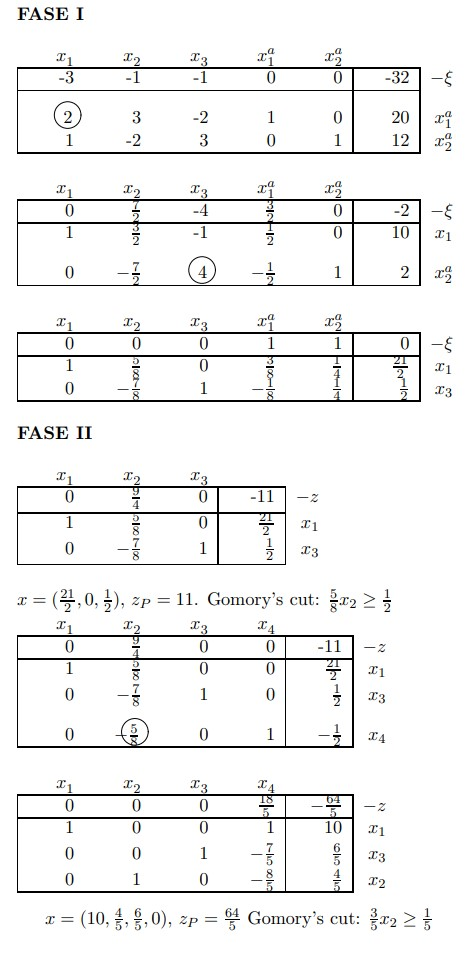
\includegraphics[width=10cm]{immagini/matrici/2_6_3_0.jpg}}
\end{center}
\begin{center}
\raisebox{-.5\height}{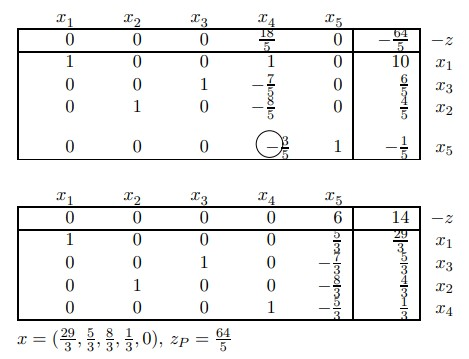
\includegraphics[width=10cm]{immagini/matrici/2_6_3_1.jpg}}
\end{center}
\subsubsection{Senstivity Analysis}
Esame 2020-02-16 Ex 2\\
\noindent\fbox{%
    \parbox{\textwidth}{%
Consider the following LP problem:\\
\begin{align*}
max:  &-5x_1 + 5x_2 + 13x_3 \\
    	&-x_1 + x_2 + 3x_3 + x_4 = 20\\
    	&12x_1 + 4x_2 + 10x_3 + x_5 = 90\\
    	&x_1,x_2,x_3,x_4,x_5 \geqq 0\\
\end{align*}

The optimal solution is $x = (0, 20, 0, 0, 10)$ with value 100\\
Given that $B^{-1} = \left[\begin{array}{cc} 1 & 0  \\ -4 & 1  \end{array} \right]$ , answer the following questions. Provide
motivations to support your arguments:\\
\begin{itemize}
		
\item what happens to the optimal base if b1, the right hand side of the
first constraint, becomes 24?
\item what happens to the optimal base if c3, the coefficient of variable
x3 becomes 10?
\end{itemize}
	}%
}%

Soluzione:\\
\\
Dalle slide del prof sulla senstivity analysis pagina 7:\\
\begin{itemize}
\item We are considering in general terms the variation of a right hand side:
\item $b \rightarrow b + \Delta b$
\item The new basic solution changes value:
\item $x_B = B^{-1} (b + \Delta b)$
\item The solution is a basic feasible solution if:
\item $x_B = B^{-1} (b + \Delta b) \geqq 0$
\item This is what we need to check in order to know if the right hand side variations let the basis feasible:
\item $B^{-1} b + B^{-1} \Delta b \geqq 0 $ , this is a new system where $\Delta b$ are the new variables.
\item $ \left[ \begin{array}{cc} 20 \\ 90  \end{array} \right] + \left[\begin{array}{cc} 1 & 0  \\ -4 & 1  \end{array} \right] * \left[ \begin{array}{cc} \Delta b_1 \\ \Delta b_2  \end{array} \right] \geqq 0$ $\Rightarrow$ $\left\{ \begin{array}{rcl} 1 \Delta b_1 + 0 \Delta b_2 \geqq -20 \\ -4 \Delta b_1 + 1 \Delta b_2 \geqq -90  \end{array}\right.$ 
\item dove: $ \left[ \begin{array}{cc} \Delta b_1 \\ \Delta b_2  \end{array} \right] $ sono la differenza dei termini noti precedenti, quindi aumentando 20 a 24:  $ \left[\begin{array}{cc} 4 \\ 0  \end{array} \right] $
\item We study what happens if only one term changes: if $ \Delta b_2 = 0$ and only $b_1$ changes:
\item $\left\{ \begin{array}{rcl}
1 \Delta b_1 \geqq -20 \\ -4 \Delta b_1 \geqq -90  \end{array}\right.$ $\Rightarrow$ $-20 \leqq \Delta b_1 \leqq \frac{90}{4}$ because originally $b_1 = -20$.
\item Fixed the other right hand sides, if $b_1$ lays between -20 and 22.5 the basis does not change, outside of this range the basis changes, so the new basis $b_1 = 24$ is outside this range, and the new solution will be different.
\end{itemize}
Per la seconda domanda, $x_3$ non è nelle soluzioni ottimali,dal testo : $x = (0, 20, 0, 0, 10)$, se poi l'abbassiamo di valore da 13 a 10 diventa pure meno appetibile per l'ottimizzazione, la soluzione quindi non cambia.

\newpage
\section{Grafi}

\subsection{GT}
Graph Theory

\subsubsection{Dijkstra}
Operiamo sempre con grafi dai costi positivi.\\
Il principio è abbastanza semplice, ogni nodo ha due indici $L[j]$ che viene pre-impostato a 0 per il nodo di partenza ed a $\infty$ e rappresenta il costo della strada più economica da $s \Rightarrow j$ mentre $pred[j]$ rappresenta il nodo precedente da cui siamo arrivati che ha la strada più economica.\\
Avremo delle etichette per ogni nodo, che hanno questi due indici e passano da temporanei a permanenti, l'esplorazione da nodo a nodo procede iterativamente selezionando sempre l'arco dal costo minore di tutti i nodi che ho raggiunto in quella fase:\\
\begin{center}
\raisebox{-.5\height}{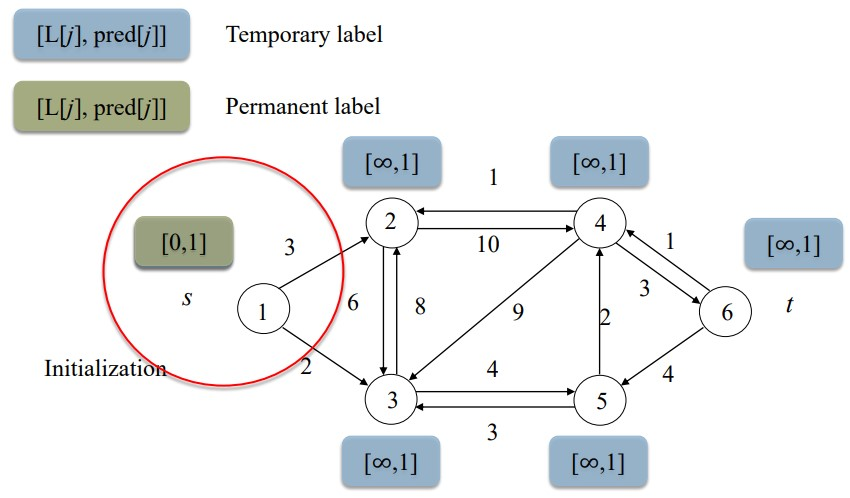
\includegraphics[width=8cm]{immagini/grafi/Dijkstra1.jpg}}
\end{center}
Etichettiamo temporaneamente i nodi che sono raggiunti da $S$,ci spostiamo al nodo che costa meno da $S$ (nodo 1 in questo caso) e approdiamo al nodo 3, essendo quello che costa meno tra i nodi già raggiunti, rendendo permanente l'etichetta perchè è oggettivamente la strada più economica, aggiungiamo anche altre etichette temporanee ai nodi che ora sono accessibili dal nodo $3$ appena esplorato, ovvero il $5$.\\

\begin{center}
\raisebox{-.5\height}{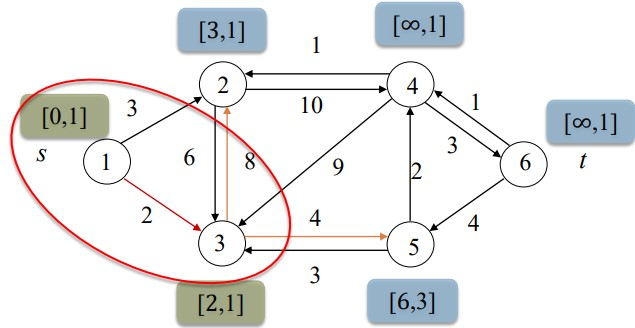
\includegraphics[width=8cm]{immagini/grafi/Dijkstra2.jpg}}
\end{center}

Rendiamo permanente anche l'etichetta del nodo 2 non avendo una strada più economica di quella trovata precedentemente ($1 \Rightarrow 2$).
Aggiungiamo un altra etichetta temporanea al nodo ora visibile dopo l'esplorazione del $2$, ovvero il $4$.\\

\begin{center}
\raisebox{-.5\height}{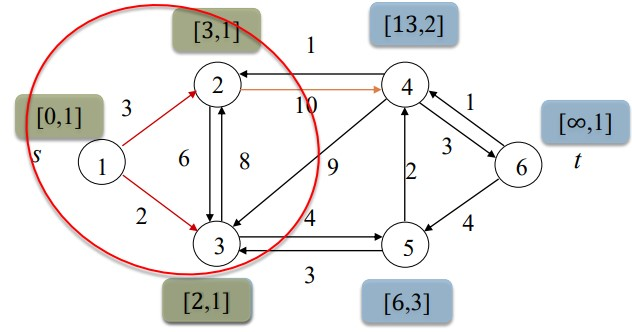
\includegraphics[width=8cm]{immagini/grafi/Dijkstra3.jpg}}
\end{center}

Mi sposto ora sul nodo $5$ essendo quello che è raggiunto da un arco che ha costo minore tra quelli disponibili e raggiunti fino ad ora, rendo l'etichetta permanente e aggiorno anche l'etichetta temporanea del nodo $4$, avendo trovato ora una strada più economica di quella precedente passante per l'attuale nodo $5$.

\begin{center}
\raisebox{-.5\height}{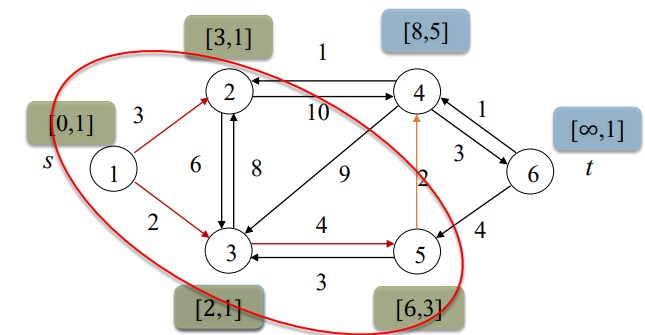
\includegraphics[width=8cm]{immagini/grafi/Dijkstra4.jpg}}
\end{center}

Ripetiamo il ragionamento per gli ultimi due veloci passaggi:

\begin{center}
\raisebox{-.5\height}{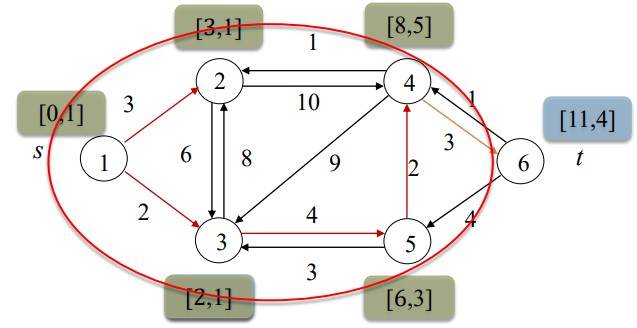
\includegraphics[width=8cm]{immagini/grafi/Dijkstra5.jpg}}
\raisebox{-.5\height}{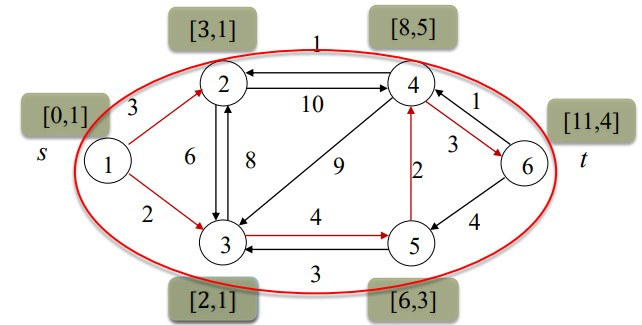
\includegraphics[width=8cm]{immagini/grafi/Dijkstra6.jpg}}
\end{center}

\subsubsection{Shortest Path Tree}
Un grafo orientato che possiamo rappresentare tramite matrice di adiacenza, può avere anche costi negativi.\\

\begin{center}
\raisebox{-.5\height}{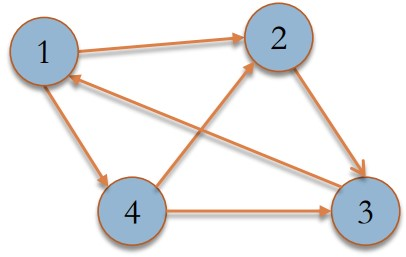
\includegraphics[width=5cm]{immagini/grafi/SPT1.jpg}}
\raisebox{-.5\height}{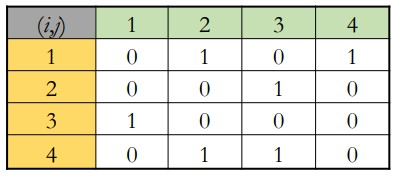
\includegraphics[width=5cm]{immagini/grafi/SPT2.jpg}}
\end{center}
Posso usare anche una lista di predecessori per rappresentarlo:\\
$S_1 = \{2,4\}$\\
$S_2 = \{3\}$\\
$S_3 = \{1\}$\\
$S_4 = \{2,3\}$\\
In forma Tabulare con due matrici, una per i  costi ed una per il nodo precedente, in questo caso sotto, $C_{ij}$ è matrice di adiacenza, mentre $L_[j]$ matrice dei pesi e $pred_[j]$ matrice dei nodi precedenti sincronizzata coi relativi costi:\\
\begin{center}
$C_{ij}=$\raisebox{-.5\height}{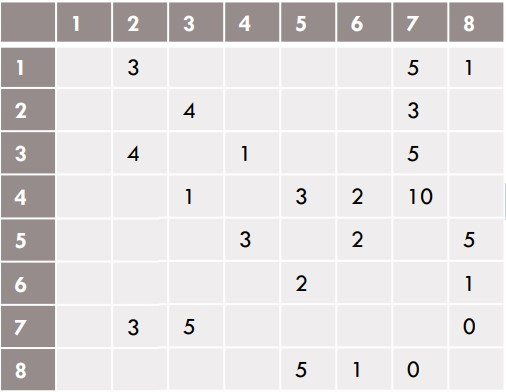
\includegraphics[width=5cm]{immagini/grafi/SPT3.jpg}}
\raisebox{-.5\height}{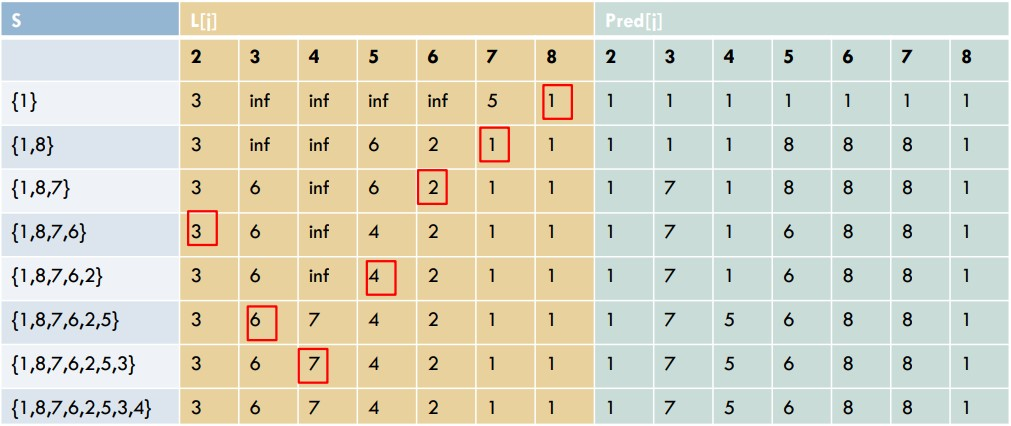
\includegraphics[width=10cm]{immagini/grafi/SPT4.jpg}}
\end{center}
\subsection{SST}
Shortest Spanning Tree
\subsubsection{Cenni di Base}
\begin{itemize}
\item \textbf{Path}(strada): Una sequenza di archi che collega due o più nodi, due nodi sono connessi se esiste almeno una path tra loro, una \textbf{simple path} è invece una strada senza ripetizione di archi
\item \textbf{Connected Graph}: se in un grafo tutti i nodi sono raggiungibili da una strada si dice che è connesso.
\item \textbf{Directed Graph}(grafo orientato): grafo che ha gli archi con frecce, ovvero indicando la direzione, la strada non è bidirezionale.
\item \textbf{Directed path}: uan sequenza consecutiva di archi che vanno dal nodo $A \Rightarrow B$.

\item \textbf{Cycl\\Circuit}(ciclo\\circuito): Se una strada di un grafo non orientato torna ad un nodo già visitato crea un ciclo, nel caso di un grafo orientato si parla invece di circuito.

\item \textbf{Complete graph}: un grafo nel quale tutti i suoi nodi sono collegati tra di loro, ovvero da ogni nodo e possibile raggiungere con un solo arco gli altri nodi.

\end{itemize}

\newpage
\subsubsection{SST Prim's}
L'algoritmo di prim's è utile per ricavare un SST da un grafo non orientato:\\
\begin{center}
\raisebox{-.5\height}{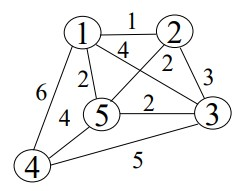
\includegraphics[width=6cm]{immagini/grafi/Prim1.jpg}}
\end{center}

Partendo dal nodo 1 che sarà usata come radice del nostro SST, costruiamo la soluzione $S=\{1\}$.\\
Marco con un $*$ l'arco che costa meno, in questo caso quello che porta al nodo $2$, e lo collego segnandomi la soluzione in $S=\{1,2\}$, segno l'arco successivo tra i nodi che ho raggiunto, in questo caso l'arco dal costo 2, che si collega al nodo $5$.

\begin{center}
\raisebox{-.5\height}{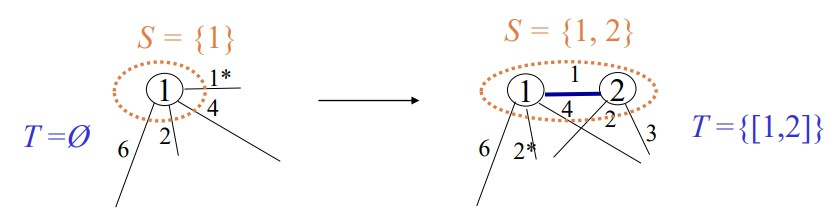
\includegraphics[width=11cm]{immagini/grafi/Prim2.jpg}}
\end{center}

Collego i nodi $1 \Rightarrow 5$ con l'arco dal costo 2 che è il minore di costo tra quelli disponibili e aggiorno la soluzione $S=\{1,2,5\}$, marco già l'arco successivo che ha costo 2.

\begin{center}
\raisebox{-.5\height}{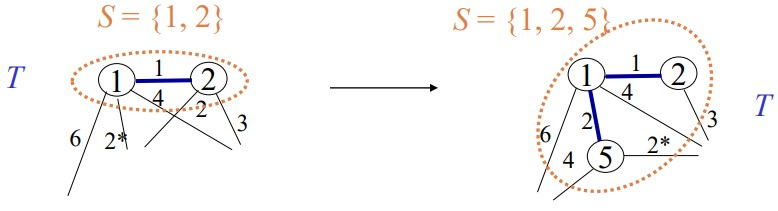
\includegraphics[width=11cm]{immagini/grafi/Prim3.jpg}}
\end{center}

Collego i nodi $5 \Rightarrow 3$, aggiorno la soluzione  $S=\{1,2,5,3\}$, marco il nodo con costo 4, ed infine lo collego nell'ultimo passaggio $5 \Rightarrow 4$, abbiamo collegato tutti i nodi, ci fermiamo e calcoliamo il costo totale che è $c(T)=9$.

\begin{center}
\raisebox{-.5\height}{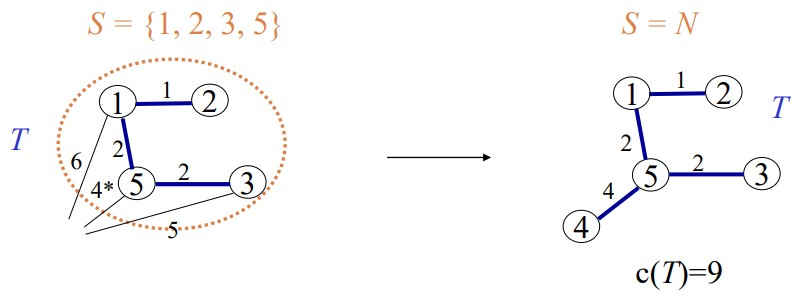
\includegraphics[width=11cm]{immagini/grafi/Prim4.jpg}}
\end{center}

\subsubsection{SST Da Matrice trovare la soluzione ottimale}
Esame 2020-06-25 Ex 2\\

\noindent\fbox{%
    \parbox{\textwidth}{%
Given the following cost matrix representing an undirected graph with 7 nodes,
find the Shortes Spanning Tree.
Provide the edges in the optimal solution and its value


\begin{center}
\raisebox{-.5\height}{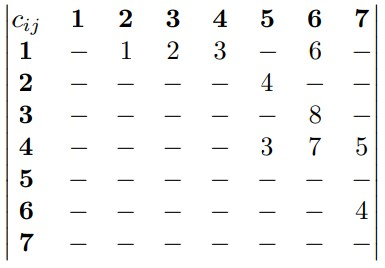
\includegraphics[width=5cm]{immagini/grafi/3_1_1_0.jpg}}
\end{center}
    }%
}%

Soluzione:\\

Si può disegnare velocemente partendo dalla matrice di adiacenza, partendo dal nodo 1, selezioni rami con il costo più basso e tiro i collegamenti, di volta in volta, la soluzione dovrà essere quella che sommando tutti i rami (senza mai passare dallo stesso nodo 2 volte) abbia il costo minore in assoluto
\\
Sol: \{(1,2), (1,3), (1,4), (4,5), (4,7), (6,7)\}\\
Cost = 18
\\

\begin{center}
\raisebox{-.5\height}{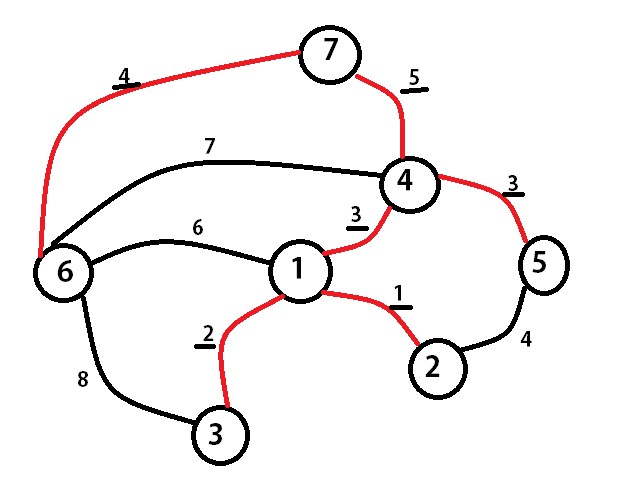
\includegraphics[width=7cm]{immagini/grafi/3_1_1_1.jpg}}
\end{center}

dal disegno, gli archi rossi son quelli selezionati per il SST, sono stati evidenziati anche i relativi pesi nel caso di stampa non a colori

\subsection{Max Flow}
Problemi di flusso, dato un grafo diretto e connesso con nodi collegati tra loro da archi, che hanno due valori, a sinistra quanto liquido sta passando (flusso), a destra quanti liquidi massimo l'arco supporta(capacità), dobbiamo trovare la strada ottimale per arrivare a destinazione.

\subsubsection{Cenni di Base}
\begin{itemize}
\item \textbf{Capacità}(Capacity): Quanto liquido può passare massimo in quell'arco
\item \textbf{Flusso}(Flow): quanto liquido sta passando effettivamente in quell'arco
\item \textbf{Flusso Accettabile}(Feasible Flow): Il flusso che scorre dal nodo $s$ $\Rightarrow$ $t$ rispetta i vincoli di capacità dei suoi archi

\item\textbf{Arco Saturato} (Saturated Arc): Arco nel quale scorre un flusso pari alla sua capacità
\item\textbf{Arco vuoto}(Empty Arc): Arco nel quale non scorre un flusso.
\item \textbf{Flusso di Conservazione} (Residual Flow): Il flusso che scorre tra più nodi deve rispettare i limiti di ogni vincolo di capacità (non sono molto sicuro su questo punto)
\item	\textbf{Taglio} (Cut): selezionando due nodi collegati tra loro, guardo la somma di capacità e/o flusso degli archi uscenti
\end{itemize}
\subsubsection{Flow Network}
Esame 2020-07-16 Ex 4\\
\noindent\fbox{%
    \parbox{\textwidth}{%
Consider the following network $G = (V, A)$, where for each arc the
current flow and the capacity are indicated as $(f_{ij} , c_{ij} )$
\begin{center}
\raisebox{-.5\height}{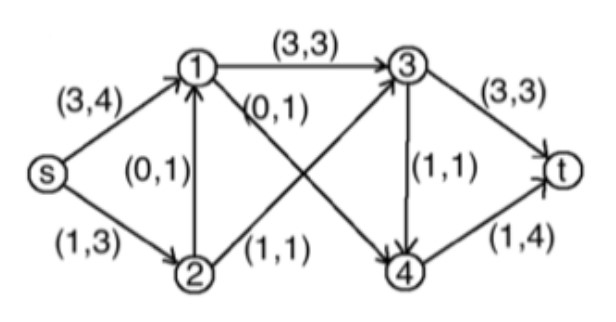
\includegraphics[width=7cm]{immagini/grafi/3_2_2_0.jpg}}
\end{center}
\begin{itemize}
\item Is the current flow feasible ? Motivate the answer.
\item Provide the value of the optimal max flow that can be carried
from s to t on the given network.
\item Provide the arcs of the corresponding minimum capacity $s-t$ cut.
\end{itemize}
    }%
}%
\\
Soluzione:
\begin{itemize}
	
\item la soluzione è accettabile, perchè tutti i flussi rispettano le capacità massime degli archi, e il flusso di conservazione, ovvero, nel nodo 4, abbiamo un output di (1,4), se per assurdo lo avessimo avuto di (4,4), per quanto avesse rispettato il vincolo di capacità, avrebbe rotto il vincolo di conservazione, perchè il nodo 4 avrebbe avuto archi entranti per un massimo di flusso dal valore 2, di conseguenza in archi uscenti il nodo 4, può avere massimo 2 di capacità reale, malgrado il suo ramo possa supportare fino a 4.\\

\begin{center}
\raisebox{-.5\height}{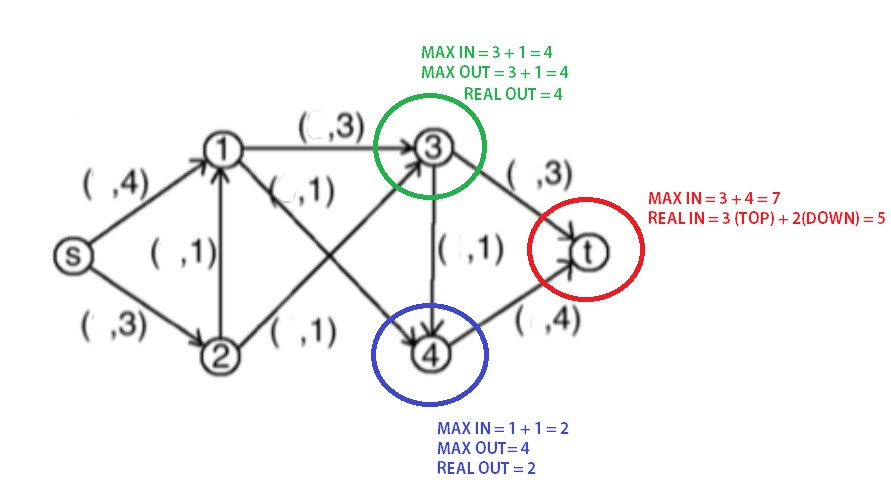
\includegraphics[width=10cm]{immagini/grafi/3_2_2_1.jpg}}
\end{center}
\item il flusso massimo che posso avere in uscita sul nodo t, è 5.\\
osservando l'immagine sopra, nel quale ho rimosso i flussi passanti e lasciato solo i flussi di capacita, notiamo che malgrado il nodo t abbia un upperbound massimo di 7, in realtà i suoi archi entranti che arrivano dal nodo 3 e 4, possono sostenere realisticamente e rispettivamente una capacità reale di uscita di 4 per il nodo 3, e di 2 per il nodo 4, dobbiamo anche notare che un nodo uscente di 3 finisce giusto nel nodo 4, quindi abbiamo nel best case scenario che il nodo 3 e 4 possono approvvigionare rispettivamente 3 dall'arco superiore e 2 dall'arco inferiore.

\item Ricordando il teorema di Ford-Fulkerson: "il valore di un flusso accettabile di un flusso massimo in un grafo è uguale alla capacità di un taglio di minima capacità", ovvero, se io faccio un taglio tra 2 nodi, che hanno capacità minima in uscita (archi uscenti), trovo la capacità massima che posso avere nel mio network, in questo caso, se prendo i nodi ($1,2$), avrò come archi uscenti {$(1,3),(1,4),(2,3)$}:
\begin{center}
\raisebox{-.5\height}{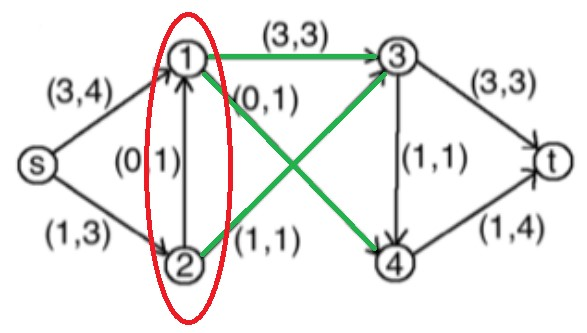
\includegraphics[width=6cm]{immagini/grafi/3_2_2_2.jpg}}
\end{center}
\end{itemize}
Questo teorema posso usarlo anche per risolvere il punto 1, ammesso il problea sia ben post rispettando tutti i vincoli
\newpage
\subsection{DP}
Dynamic Programming, usato con Knapsack e Shortest Path (Bellman-Ford)
\subsubsection{DP Knapsack 0-1 Dynamic Programming}
Esame 2021-02-16 Ex 3\\
\noindent\fbox{%
    \parbox{\textwidth}{%
Use Dynamic Programming to solve the following Knapsack Problem:
weight wj = (4, 2, 3), profit pj = (2, 1, 2), and capacity C = 5. Report
all the iterations giving the states and their values. Report the optimal
solution.
    }%
}%
\\
Soluzione: \\
per il punto 1, dobbiamo costruire 2 matrici, le colonne rappresenteranno il peso dello zaino, mentre le righe rappresentano gli oggetti, di conseguenza avremo matrici 4x6, conto una riga e colonna extra per il valore 0.\\
Una matrice rappresenterà la funzione (f) ed una l'insieme di soluzioni (j).\\
Partendo dalla matrice f, riempiamo colonna riga 0, di 0, lì non possiamo prendere niente.
\\Successivamente iteriamo per riga, partendo dalla 1, che rappresenta l'oggetto 1, ovvero $w_1=4$ e $p_1=2$, procedendo per colonne, lo possiamo inserire solo nella 4, ovvero, quando il suo peso può entrare nello zaino,svolgiamo l'algoritmo valutando se $p_j + f^{j-1}(s-w_j)>f^{j-1}(s)$ quindi, vediamo se in colonna 0 (NB. 4-4), sommandoci il profitto attuale di 2, sia un valore maggiore che quello nella riga precedente nella stessa posizione di colonna, quindi 0, se così non è, prendiamo dalla posizione $f^{j-1}(s-w_j)$ e aggiungiamo 2 come nell'immagine .\\
\\
tengo aggiornata nella seconda matrice J, gli oggetti che sto prendendo, "E" rappresenta insieme vuoto.

\raisebox{-.5\height}{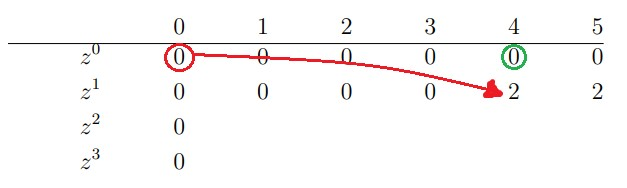
\includegraphics[width=7cm]{immagini/grafi/3_2_3_0.jpg}}
\raisebox{-.5\height}{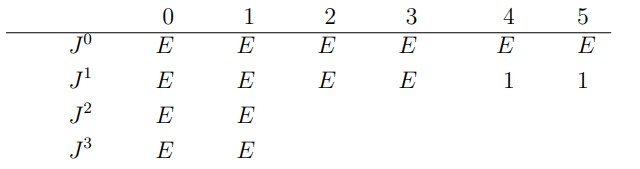
\includegraphics[width=7cm]{immagini/grafi/3_2_3_0a.jpg}}

Procedendo con la riga 2, e l'oggetto $w_2=2$ e $p_2=1$, nella colonna 2 posso inserirlo, arrivati alla colonna 4, reiterando l'algoritmo con il procedimento precedente, valuto che nella colonna 2 (NB. 4-2), della riga precedente e sommandoci il profitto di questa riga, ovvero 1, ottengo un valore più basso che prendendolo nella stessa colonna della riga precedente, proseguo quindi ricopiando quest'ultimo valore, ripeto stesso ragionamento per colonna 5.


\raisebox{-.5\height}{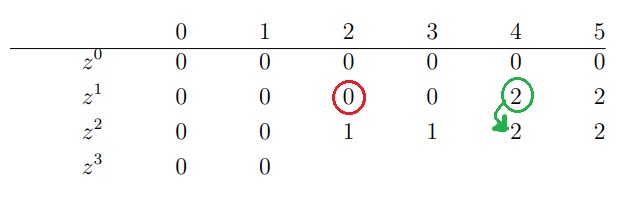
\includegraphics[width=7cm]{immagini/grafi/3_2_3_1.jpg}}
\raisebox{-.5\height}{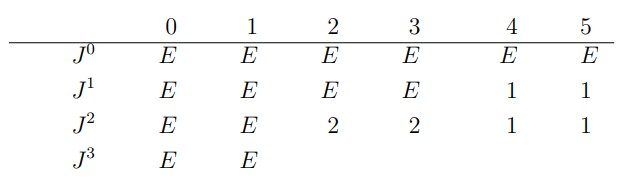
\includegraphics[width=7cm]{immagini/grafi/3_2_3_1a.jpg}}


Nell'ultima riga seguo i ragionamenti precedenti, l'oggetto $w_3=3$ e $p_3=2$, può essere inserito solamente a partire dalla 3 colonna, quindi nella colonna 2 ricopio il profitto della riga superiore, arrivati alla colonna 3, confronto che il profitto della riga superiore è inferiore a quello che avrei prendendo la colonna 0 e sommandoci il profitto di quest'ultimo oggetto, scrivo quindi 2, uguale per la colonna 4, ma posso prendere indistintamente l'oggetto 3 o 1, infine come nell'immagine qua sotto, alla colonna 5, vedo che prendendo la colonna 2 (NB. 5-3), e sommandoci il profitto attuale, ottengo un valore ancora maggiore, scrivo quindi 3.

\raisebox{-.5\height}{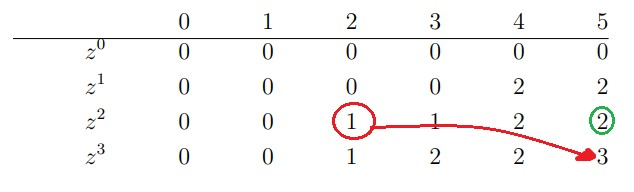
\includegraphics[width=7cm]{immagini/grafi/3_2_3_2.jpg}}
\raisebox{-.5\height}{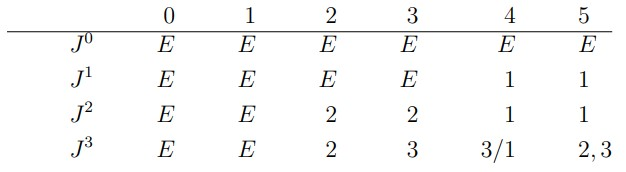
\includegraphics[width=7cm]{immagini/grafi/3_2_3_2a.jpg}}
 
 Per la seconda parte dell'esercizio dobbiamo usare l'altro algoritmo di Dynamic Programming dello knapsack.\\
 Calcoliamo il massimo proffito che sarà il nostro upperbound, sommando tutti i profitti: $\displaystyle P=\sum_{j} p_j =5$, le colonne qua rappresenteranno i profitti, le righe son le fasi, o gli oggetti come precedentemente.\\
 
Imposto nella colonna 0, tutti i valori a 0, e nella riga 0 esclusa la colonna 0, i valori ad $\infty$ (che nelle tabelle verrà rappresentato come $M$).

Per la colonna 1 ricopio $\infty$ dalla riga superiore, arrivati alla colonna 2, posso inserire il profitto del 1 oggetto $w_1=4$ e $p_1=2$, quindi scrivo 4, e riempio ad infinito il resto, aggiorno di conseguenza la seconda matrice J per indicare cosa sto prendendo come nr di oggetti.

\raisebox{-.5\height}{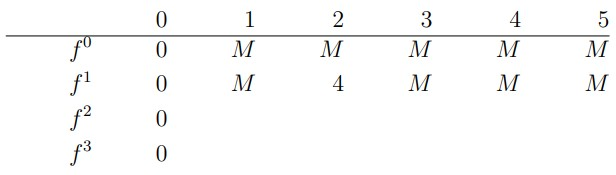
\includegraphics[width=7cm]{immagini/grafi/3_2_3_3.jpg}}
\raisebox{-.5\height}{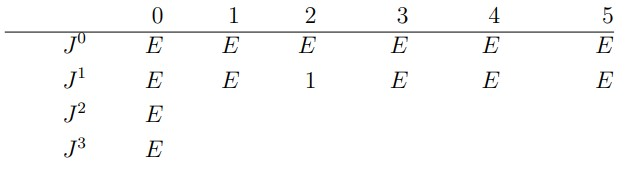
\includegraphics[width=7cm]{immagini/grafi/3_2_3_3a.jpg}}
\\
Proseguo con la 2 riga e l'oggetto $w_2=2$ e $p_2=1$, avendo profitto 1, posso inserirlo dalla prima colonna, essendo che nella posizione della riga precedente ho un $\infty$, e che l'algoritmo, simile all'es precedente, confrontando $w_j + f^{j-1}(s-p_j)<f^{j-1}(s)$, ho 0+2 = 2.\\
Nella colonna 2, mi trovo ad avere nella posizione della riga precedente un valore più basso (4) rispetto ad $\infty$ nella posizione (1,0) (ricavata dalla riga precedente e dalla colonna 2-1).\\
proseguo alla colonna 3, ricavo il 6 come valore, dalla colonna 2 (NB. 2-1) e sommandoci il peso attuale (2), scelgo il valore più basso tra le due opzioni: 6 o $\infty$  e riempio ad $\infty$ seguendo lo stesso iter il resto delle colonne.

\raisebox{-.5\height}{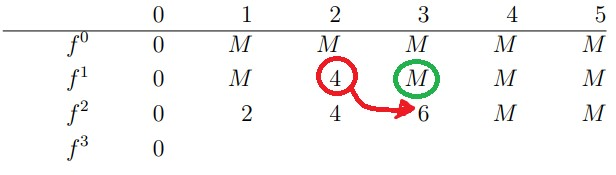
\includegraphics[width=7cm]{immagini/grafi/3_2_3_4.jpg}}
\raisebox{-.5\height}{\includegraphics[width=7cm]{immagini/grafi/3_2_3_4a.jpg}}
\\
Per l'ultima riga re-itero l'algoritmo seguendo le stesse procedure, una volta riempita la matrice, seleziono il profitto che raggiunge l'upperbound o ci va più vicino senza sforarlo, in questo caso il 5, nella posizione (3,3).

\raisebox{-.5\height}{\includegraphics[width=7cm]{immagini/grafi/3_2_3_5.jpg}}
\raisebox{-.5\height}{\includegraphics[width=7cm]{immagini/grafi/3_2_3_5a.jpg}}

\subsubsection{DP: SSP Bellman's-Ford}
\begin{center}
\raisebox{-.5\height}{\includegraphics[width=7cm]{immagini/grafi/3_2_4_0.jpg}}
\end{center}
Parto dal nodo 2, voglio sapere quale è il percorso meno costoso per arrivare ad ogni nodo!\\
Costruisco due matrici, la matrice $f$ che terrà traccia dei costi, e la matrice $pred$ che terrà traccia dei nodi precedenti in base al costo.\\
Le colonne rappresentano i nodi di arrivo, le righe sono le iterazioni ne indico $n-1$ dove n sono i nodi, li posso anche vedere come quanti archi prendo per volta per vedere i costi degli spostamenti, quindi avremo 5 righe + 1 che è quella nr 0, riempiamo nella riga 0, quella dello stato di partenza, tutto ad infinito, tranne il nodo 2, che ha un costo di 0, e la relativa colonna.
\begin{center}
\raisebox{-.5\height}{\includegraphics[width=9cm]{immagini/grafi/3_2_4_1.jpg}}
\end{center}

Analizziamo la fase 1, o riga 1, stiamo guardando i costi per arrivare al nodo 1, nella prima colonna, scrivo 2 nella matrice di $f$, ovvero il costo per arrivare dal nodo 2 al nodo 1, tengo aggiornata la matrice delle posizioni segnando 2, che è il nodo precedente da cui sono arrivato, lo stesso approccio si applica anche alle altre colonne, ad eccezione della 6, il nodo 2 non ha collegamenti diretti, quindi il costo è ignoto, mettiamo $\infty$.


\raisebox{-.5\height}{\includegraphics[width=9cm]{immagini/grafi/3_2_4_2.jpg}}
\raisebox{-.5\height}{\includegraphics[width=5cm]{immagini/grafi/3_2_4_0.jpg}}



Passiamo ora alla fase 2, nel nodo 1 posso arrivarci da 2 o da 6, 6 dalla riga precedente ha costo $\infty$, quindi riporto il costo di 2 e il percorso precedente, nella colonna 3, vedo che posso arrivare dal nodo 4, che ha costo -2, sommato al costo precedente che si trova in posizione (1,4) ottengo $4-2=2$, inserisco quindi 2, e segno il nodo 4 nella matrice prec, 6 non viene analizzato perchè ha ancora costo $\infty$.\\
Colonna 5, posso arrivarci dal nodo 6 che ignoriamo, dal 3 e dal 2 che abbiamo già segnato, vedo che dal nodo 3 ho un costo inferiore di quello precedente $6+1=7$, aggiorno di conseguenza, arrivare a 6 ora è possibile, e posso solo da 1, il costo totale sarà 4, aggiorno le matrici.


\raisebox{-.5\height}{\includegraphics[width=9cm]{immagini/grafi/3_2_4_3.jpg}}
\raisebox{-.5\height}{\includegraphics[width=5cm]{immagini/grafi/3_2_4_0.jpg}}


Per la riga 3, vedo che posso aggiornare solo la colonna 5, arrivandoci dal percorso $2 \Rightarrow 4 \Rightarrow 3 \Rightarrow 5$ a costo 1.


\raisebox{-.5\height}{\includegraphics[width=9cm]{immagini/grafi/3_2_4_5.jpg}}
\raisebox{-.5\height}{\includegraphics[width=5cm]{immagini/grafi/3_2_4_5a.jpg}}


Per la riga 4, guardando i vari costi non riusciamo ad ottenere miglioramenti eccetto per la colonna 4, con un nuovo percorso, usando 4 archi: $2 \Rightarrow 1 \Rightarrow 6 \Rightarrow 5 \Rightarrow 4$ a costo 2!


\raisebox{-.5\height}{\includegraphics[width=9cm]{immagini/grafi/3_2_4_6.jpg}}
\raisebox{-.5\height}{\includegraphics[width=5cm]{immagini/grafi/3_2_4_6a.jpg}}


Infine l'ultima riga, per la colonna 3, usando 5 archi arrivo a costo 0 con questo percorso: $2 \Rightarrow 1 \Rightarrow 6 \Rightarrow 5 \Rightarrow 4 \Rightarrow 3 $\\
il resto non trovo di meglio e rimane invariato


\raisebox{-.5\height}{\includegraphics[width=9cm]{immagini/grafi/3_2_4_7.jpg}}
\raisebox{-.5\height}{\includegraphics[width=5cm]{immagini/grafi/3_2_4_7a.jpg}}


Abbiamo trovato quindi il meno costoso per ogni nodo nell'ultima riga. 

\subsection{ILP}
Integer Linear Programming, Branch \& Bound usato con standard e knapsack. 
\subsubsection{ILP standard B\&B}
Per questo tipo di problemi usiamo il B\& B su sistemi per trovare la soluzione ottimale, è un approccio dicotomico, ogni nodo avrà due sotto problemi, selezionando una variabile frazionaria $x_j = \alpha$, ci sposteremo a sinistra impostando $x_j \leqq \lfloor \alpha \rfloor$ e a destra $x_j \geqq \lceil \alpha \rceil$\\

\begin{center}
\raisebox{-.5\height}{\includegraphics[width=6cm]{immagini/grafi/3_2_5_0.jpg}}
\end{center}

Prendiamo come esempio questo sistema:\\
\begin{align*}
max:  &x_1 + x_2 \\
    	&4x_1 - 2x_2 \geqq 1\\
    	&4x_1 + 2x_2 \leqq 11\\
    	&2x_2 \geqq 1\\
    	&x_1,x_2 integer\\
\end{align*}
Avendo variabili intere e rappresentando graficamente in problema arriviamo a questa soluzione:\\
\begin{center}
\raisebox{-.5\height}{\includegraphics[width=6cm]{immagini/grafi/3_2_5_1.jpg}}
\end{center}
All'interno del triangolo abbiamo la nostra zona ammissibile, i pallini rappresentano gli interi, ovvero dove cercheremo di avvicinarci epr raggiungere la nostra soluzione ottimale intera, facendo il gradiente, abbiamo la nostra freccia con coordinate $(1,1)$, la nostra soluzione ottimale di conseguenza è la $P^0$ con coordinata $x_1=\frac{3}{2},x_2=\frac{5}{2}$, soluzione che come abbiamo appena detto non è intera, di conseguenza, dovremmo avvicinarci al pallino nel grafico più vicino alla nostra soluzione ottimale intera.\\
La nostra soluzione con queste coordinate è $z = x_1 + x_2 \Rightarrow \frac{3}{2} + \frac{5}{2} = 4$, sarà il nostro Upper Bound (UB) di partenza del nostro albero ($P^0$), ora usando gli arrotondamenti di $\alpha$ citati prima, nel ramo sinistro arrotonderemo per difetto, in quello di destra per eccesso $x_1$, per cui:\\
\begin{center}
\raisebox{-.5\height}{\includegraphics[width=8cm]{immagini/grafi/3_2_5_2a.jpg}}
\raisebox{-.5\height}{\includegraphics[width=6cm]{immagini/grafi/3_2_5_3.jpg}}
\end{center}

Graficamente risulta così, dividiamo in sezioni per interi, a sinistra abbiamo $x_1 \leqq 1$ ed a destra abbiamo $x_1 \geqq 2$, considerato il nostro gradiente, le soluzioni ottimali delle due condizioni sono rispettivamente $z=2,5$ ricavato da $x_1 = 1, x_2=1,5$, mentre per la parte di destra abbiamo $z=3,5$ ricavato da $x_1 = 2, x_2=1,5$, ovviamente le z son state ricavate sostituendo gli $x_1,x_2$ nella funzione obbiettivo di questo problema, che ricordo è: $max:x_1+x_2$.
Vengono arrotondati per difetto le soluzioni, per le relative $P^1,P^2$ del nostro albero, non avendo ancora soluzioni intere continuiamo.\\
Non possiamo più spostarci a sx perchè andremmo sullo zero e fuori dalla zona ammissibile del problema, di conseguenza esploriamo il ramo destro:\\
\begin{center}
\raisebox{-.5\height}{\includegraphics[width=8cm]{immagini/grafi/3_2_5_4.jpg}}
\end{center}
Stiamo ora valutando $x_2$ che è anch'essa frazionaria.\\
$P^4$ esce fuori dalla zona ammissibile del problema e lo vediamo graficamente, quindi scriveremo $empty$, $P^3$ invece è nella regione ammissibile, graficamente risulta :\\
\begin{center}
\raisebox{-.5\height}{\includegraphics[width=6cm]{immagini/grafi/3_2_5_5.jpg}}
\end{center}
Avremo ancora una soluzione frazionaria, corrispondente ad $x_1 = 2,25, x_2=1$ per cui $z=3,25$, arrotondando come upperbound di $P^3$ avremo $3$, possiamo proseguire visto che la soluzione no nera ancora intera.\\

\begin{center}
\raisebox{-.5\height}{\includegraphics[width=8cm]{immagini/grafi/3_2_5_2.jpg}}
\end{center}
$P^6$ esce dalla zona accettabile, mentre $P^5$ questa volta è soluzione intera con coordinate $x_1=2,x_2=1$ e relativa $z=3$, possiamo interromperci.

\subsubsection{ILP esercizio standard B\&B}
Esame 2018-07-19 Ex 3\\
\noindent\fbox{%
    \parbox{\textwidth}{%
Consider the following PLI model:

\begin{align*}
max:  &x_1 + 4x_2 \\
    	&7x_1 - x_2 \leqq 1\\
    	&-2x_1 + x_2 \leqq 1\\
    	&2x_2 \geqq 1\\
    	&x_1,x_2 free\\
\end{align*}

Solve it with the standard Branch-and-Bound algorithm. Solve each relaxed subproblems
graphically. Perform the first branching on variable x1.
    }%
}%
\\
Soluzione: \\
Problem $P^0: x_A = (\frac{45}{11},\frac{39}{11})$ $z_A=[\frac{201}{11}]=18$\\
\begin{center}
\raisebox{-.5\height}{\includegraphics[width=9cm]{immagini/grafi/PLC1.jpg}}
\end{center}
Problem $P^1: x_B=(4,\frac{7}{2})$ $z_B=18$
\begin{center}
\raisebox{-.5\height}{\includegraphics[width=9cm]{immagini/grafi/PLC2.jpg}}
\end{center}
Problem $P^2: x_C=(4,3)$ $z_C=17$
\begin{center}
\raisebox{-.5\height}{\includegraphics[width=9cm]{immagini/grafi/PLC3.jpg}}
\end{center}
Problem $P^3: x_D=(4,3)$ $z_D=16$
\begin{center}
\raisebox{-.5\height}{\includegraphics[width=9cm]{immagini/grafi/PLC4.jpg}}
\end{center}
\begin{center}
\raisebox{-.5\height}{\includegraphics[width=7cm]{immagini/grafi/PLC5.jpg}}
\end{center}

\subsubsection{ILP esercizio B\&B 0-1}
Esame 2020-06-08 Ex 2\\
\noindent\fbox{%
    \parbox{\textwidth}{%
Consider a 0-1 knapsack problem with 5 items with profits pj = (10, 15, 8, 12, 11),
weights wj = (8, 15, 10, 17, 20) and a knapsack of size 35. Consider the
branch-and-bound used to solve the problem and the first subproblem
generated by a branching of the type xj = 0. Write the upper bound
of this subproblem, and say if the exploration must proceed to lower
levels: justify your choice.
    }%
}
\\
Soluzione:\\
Per prima cosa dobbiamo ordinare gli oggetti per $ \frac{valore}{peso} $ in ordine crescente, facendo la frazione $ \frac{pj}{wj} $, una volta ordinati, in questo esercizio è già stato fatto dal prof, calcoliamo l'Upper bound del nodo p1 con Dantzig's bound\\
\begin{center}
UB=$ \displaystyle \sum_{j=1}^{s-1} p_j + p_jx_s (\displaystyle \sum_{j=1}^{s-1} p_j + \lfloor p_j x_s \rfloor$ if integer $p_j)  $
\end{center}

\begin{center}
\raisebox{-.5\height}{\includegraphics[width=7cm]{immagini/grafi/3_2_1_0.jpg}}
\end{center}

Dalla figura vediamo che arrivati a P4, ci fermiamo che non possiamo più inserire altri oggetti, e abbiamo la nostra prima soluzione P4 = \{1,1,1,0,0\} con valore 33, risalendo a P3 ci spostiamo a dx non prendendo l'ultimo oggetto (il terzo per la precisione, valore 8 peso 10), come ogni volta che non prendiamo un oggetto, ricalcoliamo UB, in questo caso abbiamo sempre valore 33, e non ha senso esplorare ulteriormente questo ramo

\newpage
\section{GPLK}

\UseRawInputEncoding
\lstset{
  showspaces=false,
  basicstyle=\ttfamily,
  numbers=left,
  numberstyle=\tiny,
  commentstyle=\color{gray},
  breaklines=true,
  belowskip=0pt,
   tabsize=1,
  breakatwhitespace=true
}
Questa sezione si limita a raccogliere alcuni problemi in GPLK particolari senza spiegazioni.

\subsection{Dal modello al codice}
\subsubsection{Modello Easy}
Esame 2016-07-19 Ex 3\\
\noindent\fbox{%
    \parbox{\textwidth}{%
Write a GLPK or XPRESS model corresponding to the following mathematical model:\\

\begin{center}
\begin{align*}
max : z= &\displaystyle \sum_{i=1}^{n} \sum_{j=1}^{m} p_{ij} x_{ij}\\
&\displaystyle \sum_{i=1}^{n} q_ix_{ij} \leqq c &j=1,\dots,m  &  &  & (1)\\
&\displaystyle \sum_{i\in S}\sum_{j=1}^{m} x_{ij} \leqq nmy_S & i= 1,\dots,n & &j=1,\dots,m  &  (2)\\
&\displaystyle \sum_{i\notin S}\sum_{j=1}^{m} x_{ij} \leqq nmy_S & i= 1,\dots,n & &j=1,\dots,m  &  (3)\\
&x_{ij} \in \{0,1\} & i= 1,\dots,n  & & j=1,\dots,m  & (4)\\
&y_S \in \{0,1\} & & & & (5)
\end{align*}
\end{center}

   }%
}%
\\
Soluzione:\\
\begin{lstlisting}[
           language=C,
           showspaces=false,
           basicstyle=\ttfamily,
           numbers=left,
           numberstyle=\tiny,
           commentstyle=\color{gray}
        ]
param n, integer, > 0;
param m, integer, > 0;
set I := 1..n;
set J := 1..m;
set S;

param c, integer, > 0;
param p{i in I, j in J}, >= 0;
param q{i in I}, >= 0;

var x{i in I, j in J}, binary;
var ys, binary;

maximize z: sum{i in I, j in J} p[i,j]*x[i,j];

s.t. cap{j in J}: sum{i in I} q[i]*x[i,j] <= c;
yS1: sum{i in S, j in J} x[i,j] <= n*m*ys;
yS2: sum{i in I, j in J: i not in S} x[i,j] <= n*m* ys;
solve;

\end{lstlisting}

\subsubsection{Caso Particolare 1 Graffa}
Esame 2017-02-01 Ex 3\\
\noindent\fbox{%
    \parbox{\textwidth}{%
Write a GLPK or XPRESS model corresponding to the following mathematical model:\\

\begin{center}
\begin{align*}
max : z= &\displaystyle \sum_{j \in V} \sum_{i \in U} p_{ij} x_{ij} - \sum_{i \in V \backslash \{0\}} c_i y_i\\
&\displaystyle \sum_{i \in V \backslash \{n+1\}} x_{0j} \leqq 1  &  &  & (1)\\
&\displaystyle \sum_{i \in U} x_{ij} \leqq 1 & j \in V \backslash \{n+1\} & &    (2)\\
&\displaystyle \sum_{j \in V \backslash \{n+1\}} x_{ij} - \sum_{j \in U \backslash \{0\}} x_{ij} = \left\{ \begin{array}{rcl} 0 & i \in V \backslash \{0,n+1\} \\ M & i=0 \\ -M & i=n+1 \end{array}\right. & & & (3)\\
&\displaystyle \sum_{j \in V \backslash \{n+1\}} f_{ij} - \sum_{j \in U \backslash \{0\}} f_{ij} = 0 & i \in V \backslash \{0,n+1\} & & & (4)\\
&f_{ij} \leqq q_{ij}x_{ij} & i,j \in V & & & (5)\\
&x_{ij} \in \{0,1\} & \forall i \in U,j \in V  & & (6)\\
&y_j \in \{0,1\} & \forall j \in U & & & (7)\\
&f_{ij} \geqq 0 & \forall i \in U, j \in V & & (8)
\end{align*}
\end{center}
	}%
}%
\\
Soluzione:\\
\begin{lstlisting}[
           language=C,
           showspaces=false,
           basicstyle=\ttfamily,
           numbers=left,
           numberstyle=\tiny,
           commentstyle=\color{gray}
        ]
param n, integer, > 0;
param m, integer, > 0;
set V := 0..n+1;
set U := 0..n+1;
set V0 := 1..n-1;
set Vn1 := 0..n;
set V0n1 := 1..n;
set U0 := 1..n+1;
param M;

param p{i in U, j in V}, >= 0;
param q{i in U, j in V}, >= 0;
param c{i in Vn1}, >= 0;

var x{i in U, j in V}, binary;
var y{ j in V0}, binary;
var f{i in U, j in V}, >= 0;


maximize z: sum{i in U, j in V } p[i,j]*x[i,j] - sum{i in V0} c[i]*y[i];

s.t. from0: sum{j in Vn1} x[0,j] <= 1;
inj{j in Vn1}: sum{i in U} x[i,j] <= 1;
balance1x{i in V0n1}: sum{j in Vn1} x[i,j] - sum{j in U0} x[j,i] = 0;
balance2x: sum{j in Vn1} x[0,j] - sum{j in U0} x[j,0] = M;
balance3x: sum{j in Vn1} x[n+1,j] - sum{j in U0} x[j,n+1] = -M;
balance1f{i in V0n1}: sum{j in Vn1} f[i,j] - sum{j in U0} f[j,i] = 0;
fx{i in V, j in V}: f[i,j] - q[i,j]*x[i,j] <= 0;
solve;


\end{lstlisting}

\subsubsection{Caso Particolare 2 Sommatoria doppio insieme}
Esame 2017-06-29 Ex 3\\
\noindent\fbox{%
    \parbox{\textwidth}{%
Write a GLPK or XPRESS model corresponding to the following mathematical model:\\

\begin{center}
\begin{align*}
min : z= &\displaystyle \sum_{j = 1}^{n}c_{ij} x_{0j}\\
&\displaystyle \sum_{j=1}^{n+1} x_{0j} - \sum_{j=0}^{n} x_{j,n+1} = 0  &  &  & (1)\\
&\displaystyle \sum_{j=0}^{n+1} x_{ij} - \sum_{j=0}^{n+1} x_{ji} = 0 &i=1,\dots,n & &    (2)\\
&\displaystyle  \sum_{i=0, i \notin S_k}^{n+1} x_{ij}  \sum_{j \in S_k} x_{ij} \leqq 1 &k=1,\dots,p  & & (3)\\
&\displaystyle \sum_{i \in S_k} \sum_{j \in S_k} x_{ij} \geqq 1 &k=1,\dots,p  & & (4)\\
&x_{ij} \in \{0,1\} &i,j = 0,\dots,n+1,i \neq j  & & (5)
\end{align*}
\end{center}
	}%
}%
\\
Soluzione:\\
\begin{lstlisting}[
           language=C,
           showspaces=false,
           basicstyle=\ttfamily,
           numbers=left,
           numberstyle=\tiny,
           commentstyle=\color{gray}
        ]
param n, integer, > 0;
param p, integer, > 0;

set I := 0..n+1;
set Ip := 1..n;
set P := 1..p;
set S{k in P};

param q{i in I}, >= 0;
param c{i in I, j in I}, >= 0;

var x{i in I, j in I}, >= 0, binary;


minimize z: sum{j in I} c[0,j]* x[0,j];

s.t.
V1: sum{j in I: j != 0} x[0,j] - sum{j in I: j != n+1} x[j,n+1] = 0;
V2{i in Ip}: sum{j in I} x[i,j] - sum{j in I} x[j,i] = q[i];
V3{k in P}: sum{i in I diff S[k], j in S[k]} x[i,j] <= 1;
V4{k in P}: sum{i in S[k], j in S[k]} x[i,j] >= 1;
solve;

\end{lstlisting}


\subsection{Dal codice al modello}
\subsubsection{Normale}
Esame 2017-02-17 Ex 3\\

 Consider the following GLPK program and write the corresponding
mathematical model.\\
\begin{lstlisting}[
           language=C,
           showspaces=false,
           basicstyle=\ttfamily,
           numbers=left,
           numberstyle=\tiny,
           commentstyle=\color{gray}
        ]
param n, integer, > 0;
param m, integer, > 0;
set V := 0..n;
set U := 0..n;
set V1 := 1..n;
set U1 := 1..n;
set UU{i in U};

param c{i in U, j in V}, >= 0;
param s{i in U1}, >= 0;
param q{i in U, j in V}, >= 0;

var x{i in U, j in V}, binary;
var y{ j in U1}, binary;
var f{i in U, j in V}, >= 0;

maximize z: sum{i in U, j in V } c[i,j]*x[i,j] - sum{i in U1} s[i]*y[i];
s.t. TO0: sum{j in V} x[j,0] <= 1;
balance{i in U1}: sum{j in V1} x[i,j] - sum{j in U1} x[j,i] = 0;
FandX{i in V, j in V}: f[i,j] - q[i,j]*x[i,j] <= 0;
XandY{i in U1}: sum{j in V} x[i,j] <= sum{j in V} q[i,j]*y[i];
ContrUsubset{i in U}: sum{j in UU[i]} x[i,j] <= 1;
solve;
\end{lstlisting}

Soluzione:\\
\begin{center}
\begin{align*}
max : z= &\displaystyle \sum_{i=0}^{n} \sum_{j=0}^{n} c_{ij} x_{ij} + \sum_{i=0}^{n} s_i y_i\\
&\displaystyle \sum_{j=0}^{n} x_{j0} \leqq 1  &  &  & (1)\\
&\displaystyle \sum_{j=01}^{n} x_{ij} - \sum_{j=1}^{n} x_{ji} = 0 & i=1,\dots,n & &    (2)\\
&\displaystyle f_{ij} - q_{ij}x_{ij} \leqq 0 & i,j = 0,\dots,n & & & (3)\\
&\displaystyle \sum_{j=0}^{n} x_{ij} \leqq \sum_{j=0}^{n} q_{ij} y_i & i= 1,\dots,n  & & (4)\\
&\displaystyle \sum_{j \in UU_i} x_{ij} \leqq 1 & i= 0,\dots,n & & (5)\\
&x_{ij} \in \{0,1\} & i,j=0,\dots,n  & & (6)\\
&y_i \in \{0,1\} & i=1,\dots,n & & & (7)\\
&f_{ijt} \geqq 0 & i,j=0,\dots,n & & (8)
\end{align*}
\end{center}

\section{Domande varie di teoria}
Ricordo che il prof assegna +1 a risposta corretta, ma toglie -1 a risposta errata!, può essere che alcune domande abbiano più di una risposta corretta o nessuna risposta.\\
Per alcune purtroppo non ho soluzione certa
\subsection{PLC degenerate}
\noindent\fbox{%
    \parbox{\textwidth}{%
A basic solution of a PLC problem is called degenerate when: (a) there are more variables
than constraints; (b) the number of basic variables with zero value is equal to the number of
constraints; (c) the number of basic variables with zero value is equal to the difference of the
number of columns and rows (n − m); (d) the number of basic variables with non-zero value is
equal to the number of rows in the constrains matrix; (e) the basic matrix is invertible.
}%
}%
\\
Soluzione:\\
Nessuna di queste è giusta.
\subsection{PLC sensitivty}
\noindent\fbox{%
    \parbox{\textwidth}{%
Given a PLC problem the sensitivity analysis of a right hand side value b: (a) defines an
upper bound on the optimal solution value; (b) defines the minimum and maximum value of
b which does not change the optimal basis; (c) defines the minimum and maximum value of b
which does not change the value of the optimal solution; (d) defines the range of values of b
which does not change the reduced costs; (e) defines the range of values of b which does not
change the dual variables;
}%
}%
\\
Soluzione:\\
(B)
\subsection{B\&B}
\noindent\fbox{%
    \parbox{\textwidth}{%
 The branch-and-bound method: (a) is used to find the computational complexity of the
problem; (b) can be applied to minimization problems in standard form; (c) finds the optimal
solution of an NP-complete problem; (d) always use as bounding procedure the solution of a
PLC problem; (e) none of the above answers.
}%
}%
\\
Soluzione:\\
(C)
\subsection{PLC minimization}
\noindent\fbox{%
    \parbox{\textwidth}{%
Given a PLC problem P in minimization form, with 2 constraints with sign ’≥’ and 1
constraint with sign ’=’, and 5 variables, consider the dual problem D: (a) D has 3 variables
and 5 constraints; (b) D has 5 variables and 3 constraints; (c) the first variable of D must be
non-negative; (d) the third variable of D is unrestricted in sign; (e) the second variable of D
must be non-positive.
}%
}%
\\
Soluzione:\\
(A,C,D)
\subsection{cutting Plane}
\noindent\fbox{%
    \parbox{\textwidth}{%
The cutting plane method: (a) is used to solve linear programming problems with continuous variables; (b) terminates in a polynomial number of iterations; (c) is used to solve
NP-complete (”difficult”) problems; (d) at each iteration uses the simplex algorithm to solve
the current subproblem; (e) uses the lowest-first strategy to explore the subproblems.
}%
}%
\\
Soluzione:\\
(C,D)
\subsection{PLC dual}
\noindent\fbox{%
    \parbox{\textwidth}{%
Given a primal PLC problem in minimization form and its dual: (a) if the primal has finite solution, then the dual has finite solution; (b) a feasible dual solution may have a value smaller than that of the optimal primal solution; (c) if the primal is unbounded, then the dual is unbounded; (d) any feasible solution of the primal has a value greater or equal to any feasible solution of the dual; (e) if the primal is empty, then the dual is empty.
}%
}%
Soluzione:\\
(A,B,D)

\subsection{Dijkstra}
\noindent\fbox{%
    \parbox{\textwidth}{%
The Dijkstra algorithm : (a) cannot be used in a graph with negative cost arcs; (b) cannot be used in a graph with negative circuits; (c) can be used to find the shortest path in a directed graph, from a source node to a sink node; (d) can be used to find the minimum cost spanning tree; (e) cannot be applied to acyclic graphs.
}%
}%
Soluzione:\\
(A,B,C)

\subsection{B\&B knapsack}
\noindent\fbox{%
    \parbox{\textwidth}{%
The branch-and-bound method for 0-1 knapsack problems: (a) uses a decision tree with an exponential number of levels; (b) uses a decision tree with a polynomial number of levels; (c) uses the lowest-first strategy to explore the decision tree; (d) computes an upper bound at each node of the decision tree; (e) uses a decision tree with an exponential number of nodes.
}%
}%
Soluzione:\\
(B,E)

\subsection{Branch \& cut}
\noindent\fbox{%
    \parbox{\textwidth}{%
The branch-and-cut method: (a) is used to solve linear programming problems with continuous variables; (b) always uses the lowest-first strategy to explore the subproblems.; (c) is used to solve NP-complete (“difficult”) problems; (d)  terminates in a polynomial number of iterations; (e) at each iteration uses the simplex algorithm to solve the current subproblem.
}%
}%
Soluzione:\\
(C,E)
\subsection{PLC}
\noindent\fbox{%
    \parbox{\textwidth}{%
Given a PLC problem with $n$ variables and $m$ constraints, a basic matrix is: (a) a collection of $m$ constraints; (b) none of the above answers.; (c) a square $m$x$m$ matrix with value 1 on the main diagonal; (d) a collection of $n-m$ columns of the constraint matrix; (e) a square submatrix of the constraint matrix, that can be inverted.
}%
}%
Soluzione:\\
(B)
\end{document}
